\title[DS - Time,clocks,events]{\textbf{Distributed Algorithms}\\Time, clocks and the ordering of events}

\begin{document}

\begin{frame}
\titlepage
\end{frame}

\section{Modeling Distributed Executions}

\begin{frame}{Distributed Execution}

\begin{definition}[Distributed algorithm]
A \alert{distributed algorithm} is a collection of distributed automata,
one per process
\end{definition}
\vfill
\begin{definition}[Distributed execution]
	The \alert{execution} of a distributed algorithm is a sequence of \alert{events} executed
  by the processes
  \BI
  \item \alert{Partial execution}: a finite sequence of events
  \item \alert{Infinite execution}: a infinite sequence of events
  \EI
\end{definition}
\vfill
\begin{block}{Possible events}
  \BI
   \item $\send(m,p)$: sends a message $m$ to process $p$
   \item $\receive(m)$: receives a message $m$
   \item {\em local events} that change the local state
  \EI
\end{block}
\end{frame}

\subsection{Histories}

\begin{frame}{Histories}
	
\begin{definition}[Local history]
The \alert{local history} of process $p_i$ is a (possibly infinite)
  sequence of events $h_i = e^0_i e^1_i e^2_i \ldots e^{m_i}_i$ (\emph{canonical enumeration})
\end{definition}
\vfill
\begin{definition}[Partial history]
The \alert{partial history} up to event $e^k_i$ is denoted $h^k_i$ and
  is given by the prefix of the first $k$ events of $h_i$
\end{definition}
\vfill
% \begin{definition}[Global history]
% The \emph{global history} is given by the union of the events belonging
% to the local histories:
% \[
%   H = h_1 \cup h_2 \cup \ldots \cup h_n
% \]
%\end{definition}

\end{frame}

\begin{frame}{Histories}

\BIL
\item Local histories do not specify any relative timing between events
  belonging to different processes.
\item We need a notion of ordering between events, that could help
  us in deciding whether:
  \BI
  \item one event occurs before another
  \item they are actually concurrent
  \EI
\EIL

\end{frame}

\subsection{Happen-before}

\begin{frame}{Happen-Before}

\begin{definition}[Happen-before]
We say that an event $e$ \alert{happens-before} an event $e'$, and write \alert{$e \rightarrow e'$}, if one of the following three cases is true:
\BE
\item $\exists p_i \in \Pi: e = e_i^r, \quad e'=e_i^s, \quad r<s$ \\
  (if $e$ and $e'$ are executed by the same process, $e$ before $e'$)
\item $e = \send(m) \wedge e' = \receive(m)$ \\
  (if $e$ is the send event of a message $m$ and $e'$ is the corresponding
   receive event)
\item $\exists e'': e \rightarrow e'' \rightarrow e')$ \\
  (in other words, $\rightarrow$ is transitive)
\EE
\end{definition}
 
\end{frame}

\begin{frame}{Space-Time Diagram of a Distributed Computation}

\begin{figure} 
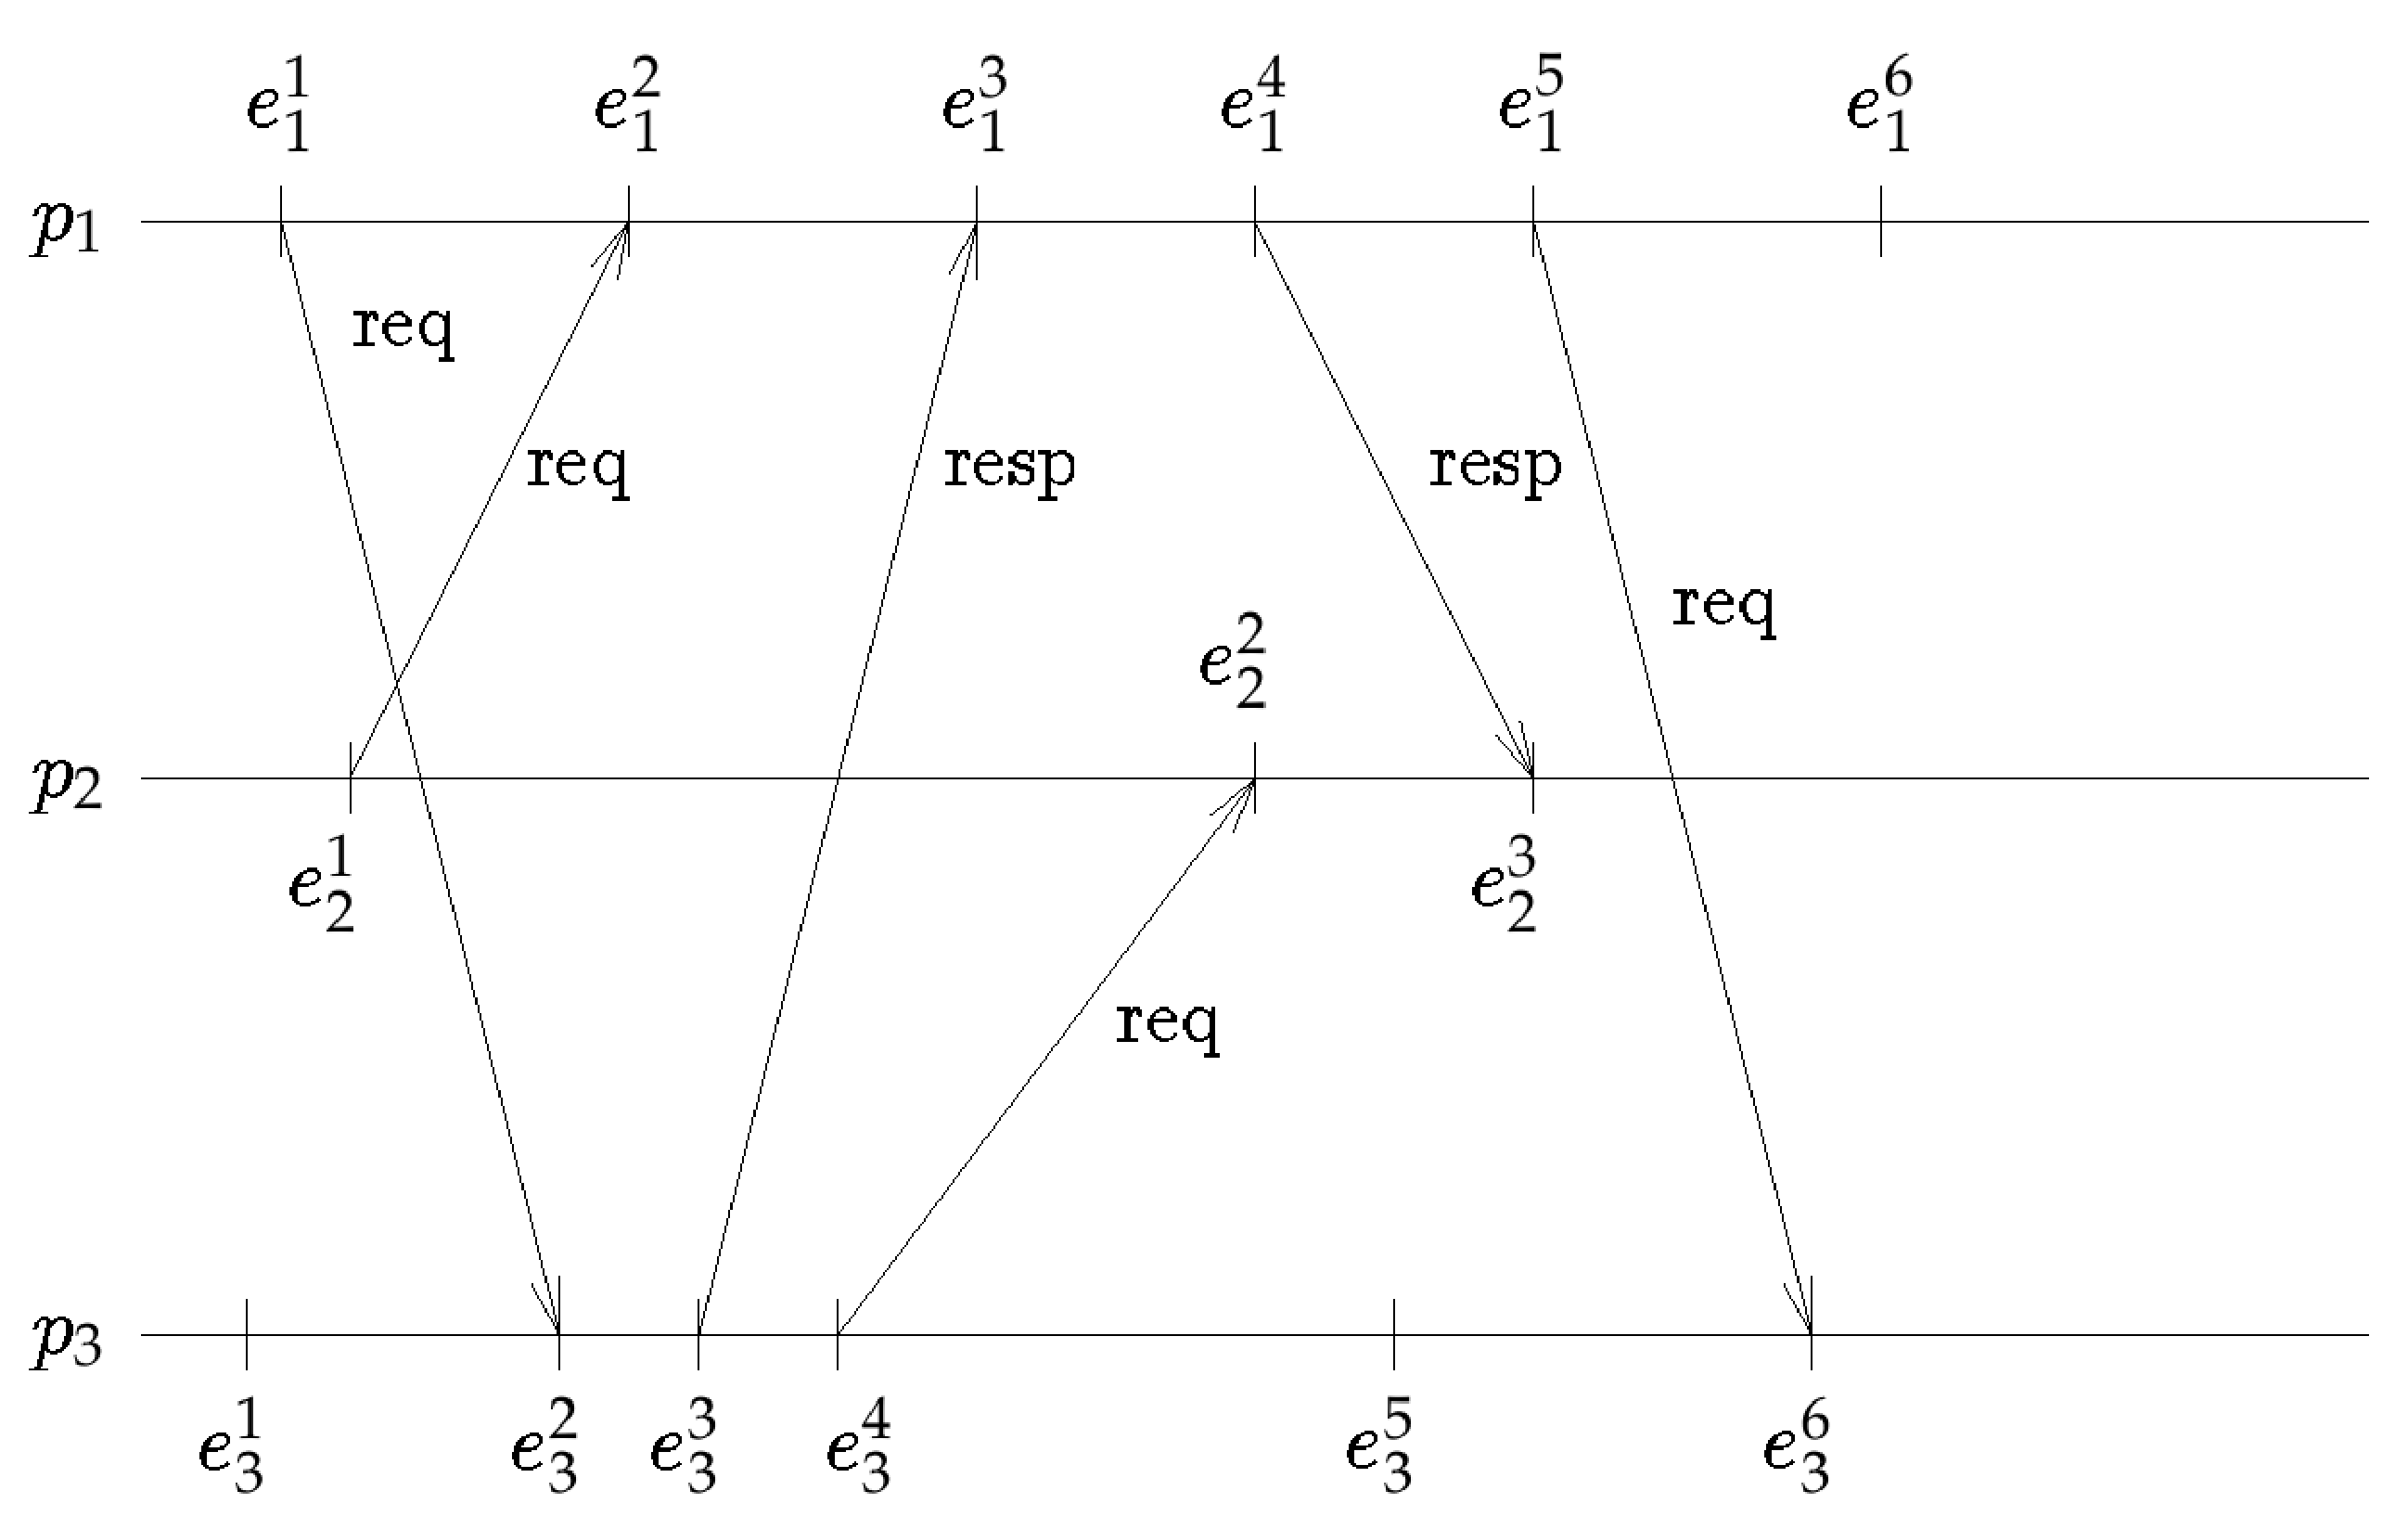
\includegraphics[width=10cm]{figs/02/figure-1}
\end{figure}	

\end{frame}


\begin{frame}{Meaning of Happen-Before}

If $e \rightarrow e'$, this means that we can find a series of events
$e^1 e^2 e^3 \ldots e^n$, where $e^1 = e$ and $e^n = e'$, such that
for each pair of consecutive events $e^i$ and $e^{i+1}$:
\BE
\item $e^i$ and $e^{i+1}$ are executed on the same process, in this order
\item $e^i = \send(m)$ and $e^{i+1} = \receive(m)$
\EE

\bigskip
\structure{Notes:}
\BIL
\item {\em happen-before} captures the concept of \alert{potential causal ordering}
\item {\em happen-before} captures a flow of data between two events.
\item Two events $e,e'$ that are not related by the happen-before relation 
  ($e \not\rightarrow e' \wedge e' \not\rightarrow e$) are \alert{concurrent},
  and we write $e || e'$.
\EIL

\end{frame}

\begin{frame}{Homework}

Prove or disprove that the $||$ relation is transitive.

\end{frame}



\begin{frame}{Reality check}

\begin{block}{Forse non tutti sanno che...}
The multi-threaded memory model of Java is based on the happen-before relation,
where communication between threads is based on the acquisition and release of
locks.

\bigskip
\url{http://download.oracle.com/javase/6/docs/api/java/util/concurrent/package-summary.html}
\end{block}

	
\end{frame}


\subsection{Global states and cuts}

\begin{frame}{Global States}
	
\begin{definition}[Local state]
\BI
\item The \alert{local state} of process $p_i$ after the execution of
  event $e_i^k$ is denoted $\sigma_i^k$
\item The local state contains all data items accessible by that process
\item Local state is completely private to the process
\item $\sigma_i^0$ is the \alert{initial state} of process $p_i$
\EI
\end{definition}
\bigskip
\begin{definition}[Global state]
The \alert{global state} of a distributed computation is an $n$-tuple of local
  states $\Sigma = (\sigma_1, \ldots, \sigma_n)$, one for each process.
\end{definition}

\end{frame}

\begin{frame}{Cut}

\begin{definition}[Cut]
A \alert{cut} of a distributed computation is the union of $n$ partial
  histories, one for each process:
\[
  C = h_1^{c_1} \cup h_2^{c_2} \cup \ldots \cup h_n^{c_n}
\]
\end{definition}

\bigskip
\BIL
\item A cut may be described by a tuple $(c_1, c_2, \ldots, c_n)$, 
  identifying the \alert{frontier} of the cut, i.e. the set of last events,
  one per process.
\item Each cut $(c_1, \ldots, c_n)$ has a corresponding global state
$(\sigma_1^{c_1}, \sigma_2^{c_2}, \ldots, \sigma_n^{c_n})$.
\EIL
\end{frame}

\begin{frame}{Cuts}

\begin{figure} 
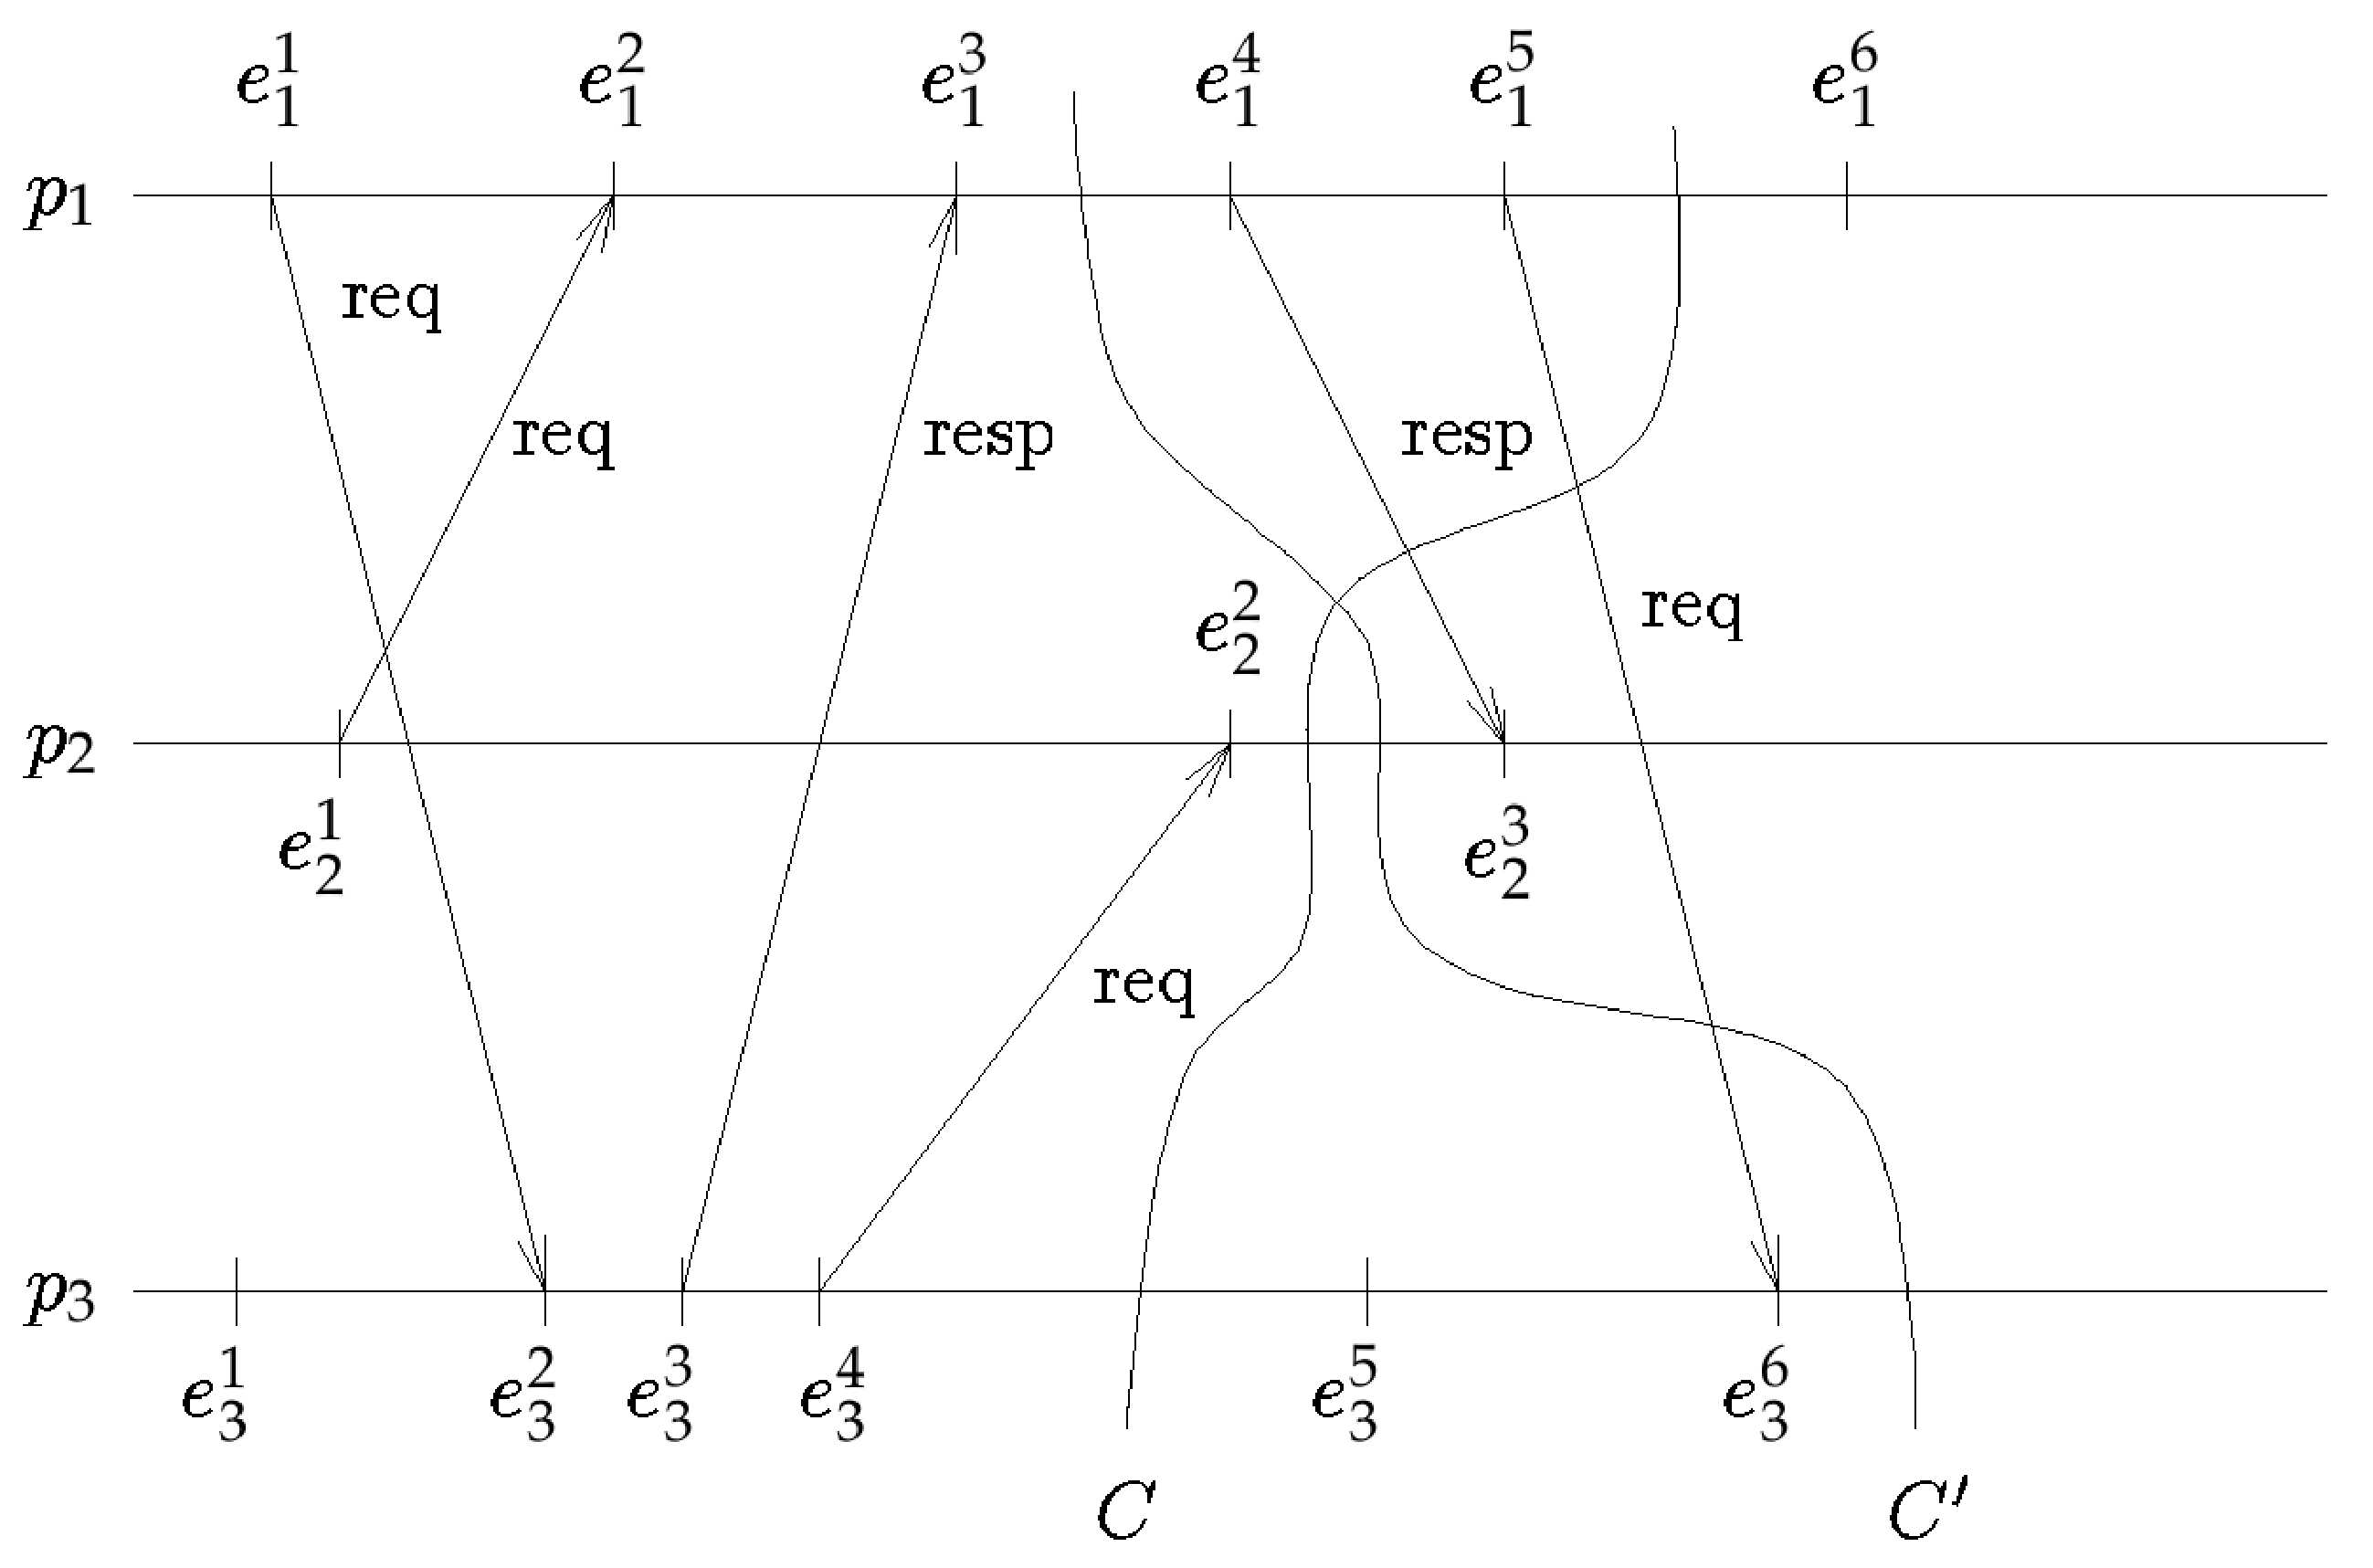
\includegraphics[width=10cm]{figs/02/figure-2}
\end{figure}
\end{frame}

\begin{frame}{Consistent cut}

Consider cuts $C'$ and $C$ in the previous figure.
\BIL
\item Is it possible that cut $C$ correspond to a ``real'' state in the
  execution of a distributed algorithm?
\item Is it possible that cut $C'$ correspond to a ``real'' state in the
  execution of a distributed algorithm?
\EIL
\end{frame}

\begin{frame}{Consistent cut}

\begin{definition}[Consistent cut]
A cut $C$ is \alert{consistent} is for all events $e$ and $e'$,
\[
  (e \in C) \wedge (e' \rightarrow e) \Rightarrow e' \in C
\]
\end{definition}

\begin{definition}[Consistent global state]
A global state is \alert{consistent} if the corresponding cut is consistent.
\end{definition}

\medskip
In other words: 
\BI
  \item A consistent cut is left-closed w.r.t. the happen-before relation
  \item All messages that have been received must have been sent before
\EI

\end{frame}



\begin{frame}{Consistent cut}

\BI
\item In the previous figures, $C$ is consistent and $C'$ is not.
\item In the space-time diagram, a cut $C$ is consistent if all
  the arrows start on the left of the cut and finish on the right
  of the cut.
\item Consistent cuts represent the concept of scalar time in distributed
  computation: it is possible to distinguish between a ``before'' and
  an ``after''.
\item \alert{Predicates} can be evaluated in consistent cuts, because they correspond
to potential global states that could have taken place during an execution.
\EI
\end{frame}


%%%%%%%%%%%%%%%%%%%%%%%%%%%%%%%%%%%%%%%%%%%%%%%%%%%%%%%%%%%%%%%%%%%%%

\section{Global predicate evaluation}

\subsection{Problem definition}

\begin{frame}{Introduction}

\begin{definition}[Global Predicate Evaluation]
The problem of detecting whether the global state of a distributed system satisfies
some predicate $\Phi$.
\end{definition}

\bigskip
\structure{Motivation}
\BIL
\item Many important distributed problems require to react when when the global
  state of the system satisfies a given condition.
  \BI
  \item \alert{Monitoring}: Notify an administrator in
    case of failures
  \item \alert{Debugging}: Verify whether an invariant 
    is respected or not
  \item \alert{Deadlock detection}: can the computation continue?
  \item \alert{Garbage collection}: like Java, but distributed
  \EI
\item Thus, the \emph{ability to construct a global state} and 
  evaluate a predicate over it is a core
  problem in distributed computing.
\EIL
\end{frame}

\begin{frame}{Examples}

\begin{figure} 
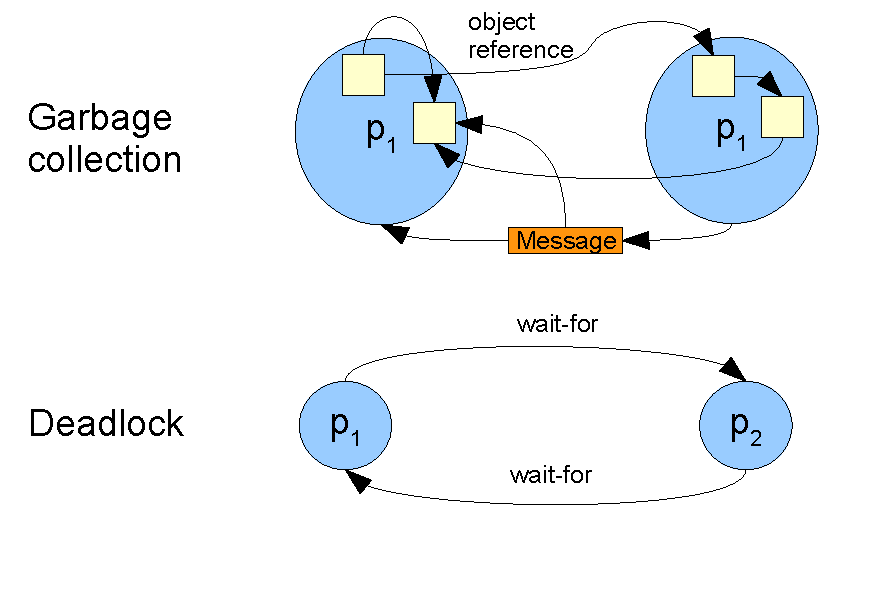
\includegraphics[width=11cm]{figs/03/gpe}
\end{figure}

\end{frame}


\begin{frame}{Why GPE is difficult}

A global state obtained through remote observations could be
\BIL
\item \alert{obsolete}: represent an old state of the system. \\
  \emph{Solution}: build the global state more frequently
\item \alert{inconsistent}: capture a global state that could never
  have been occurred in reality\\
  \emph{Solution}: build only consistent global states
\item \alert{incomplete}: not ``capture'' every moment of the system\\
  \emph{Solution}: build all possible consistent global states
\EIL
\end{frame}

\subsection{Example: deadlock detection}

\begin{frame}{Space-Time Diagram of a Distributed Computation}

\begin{figure} 
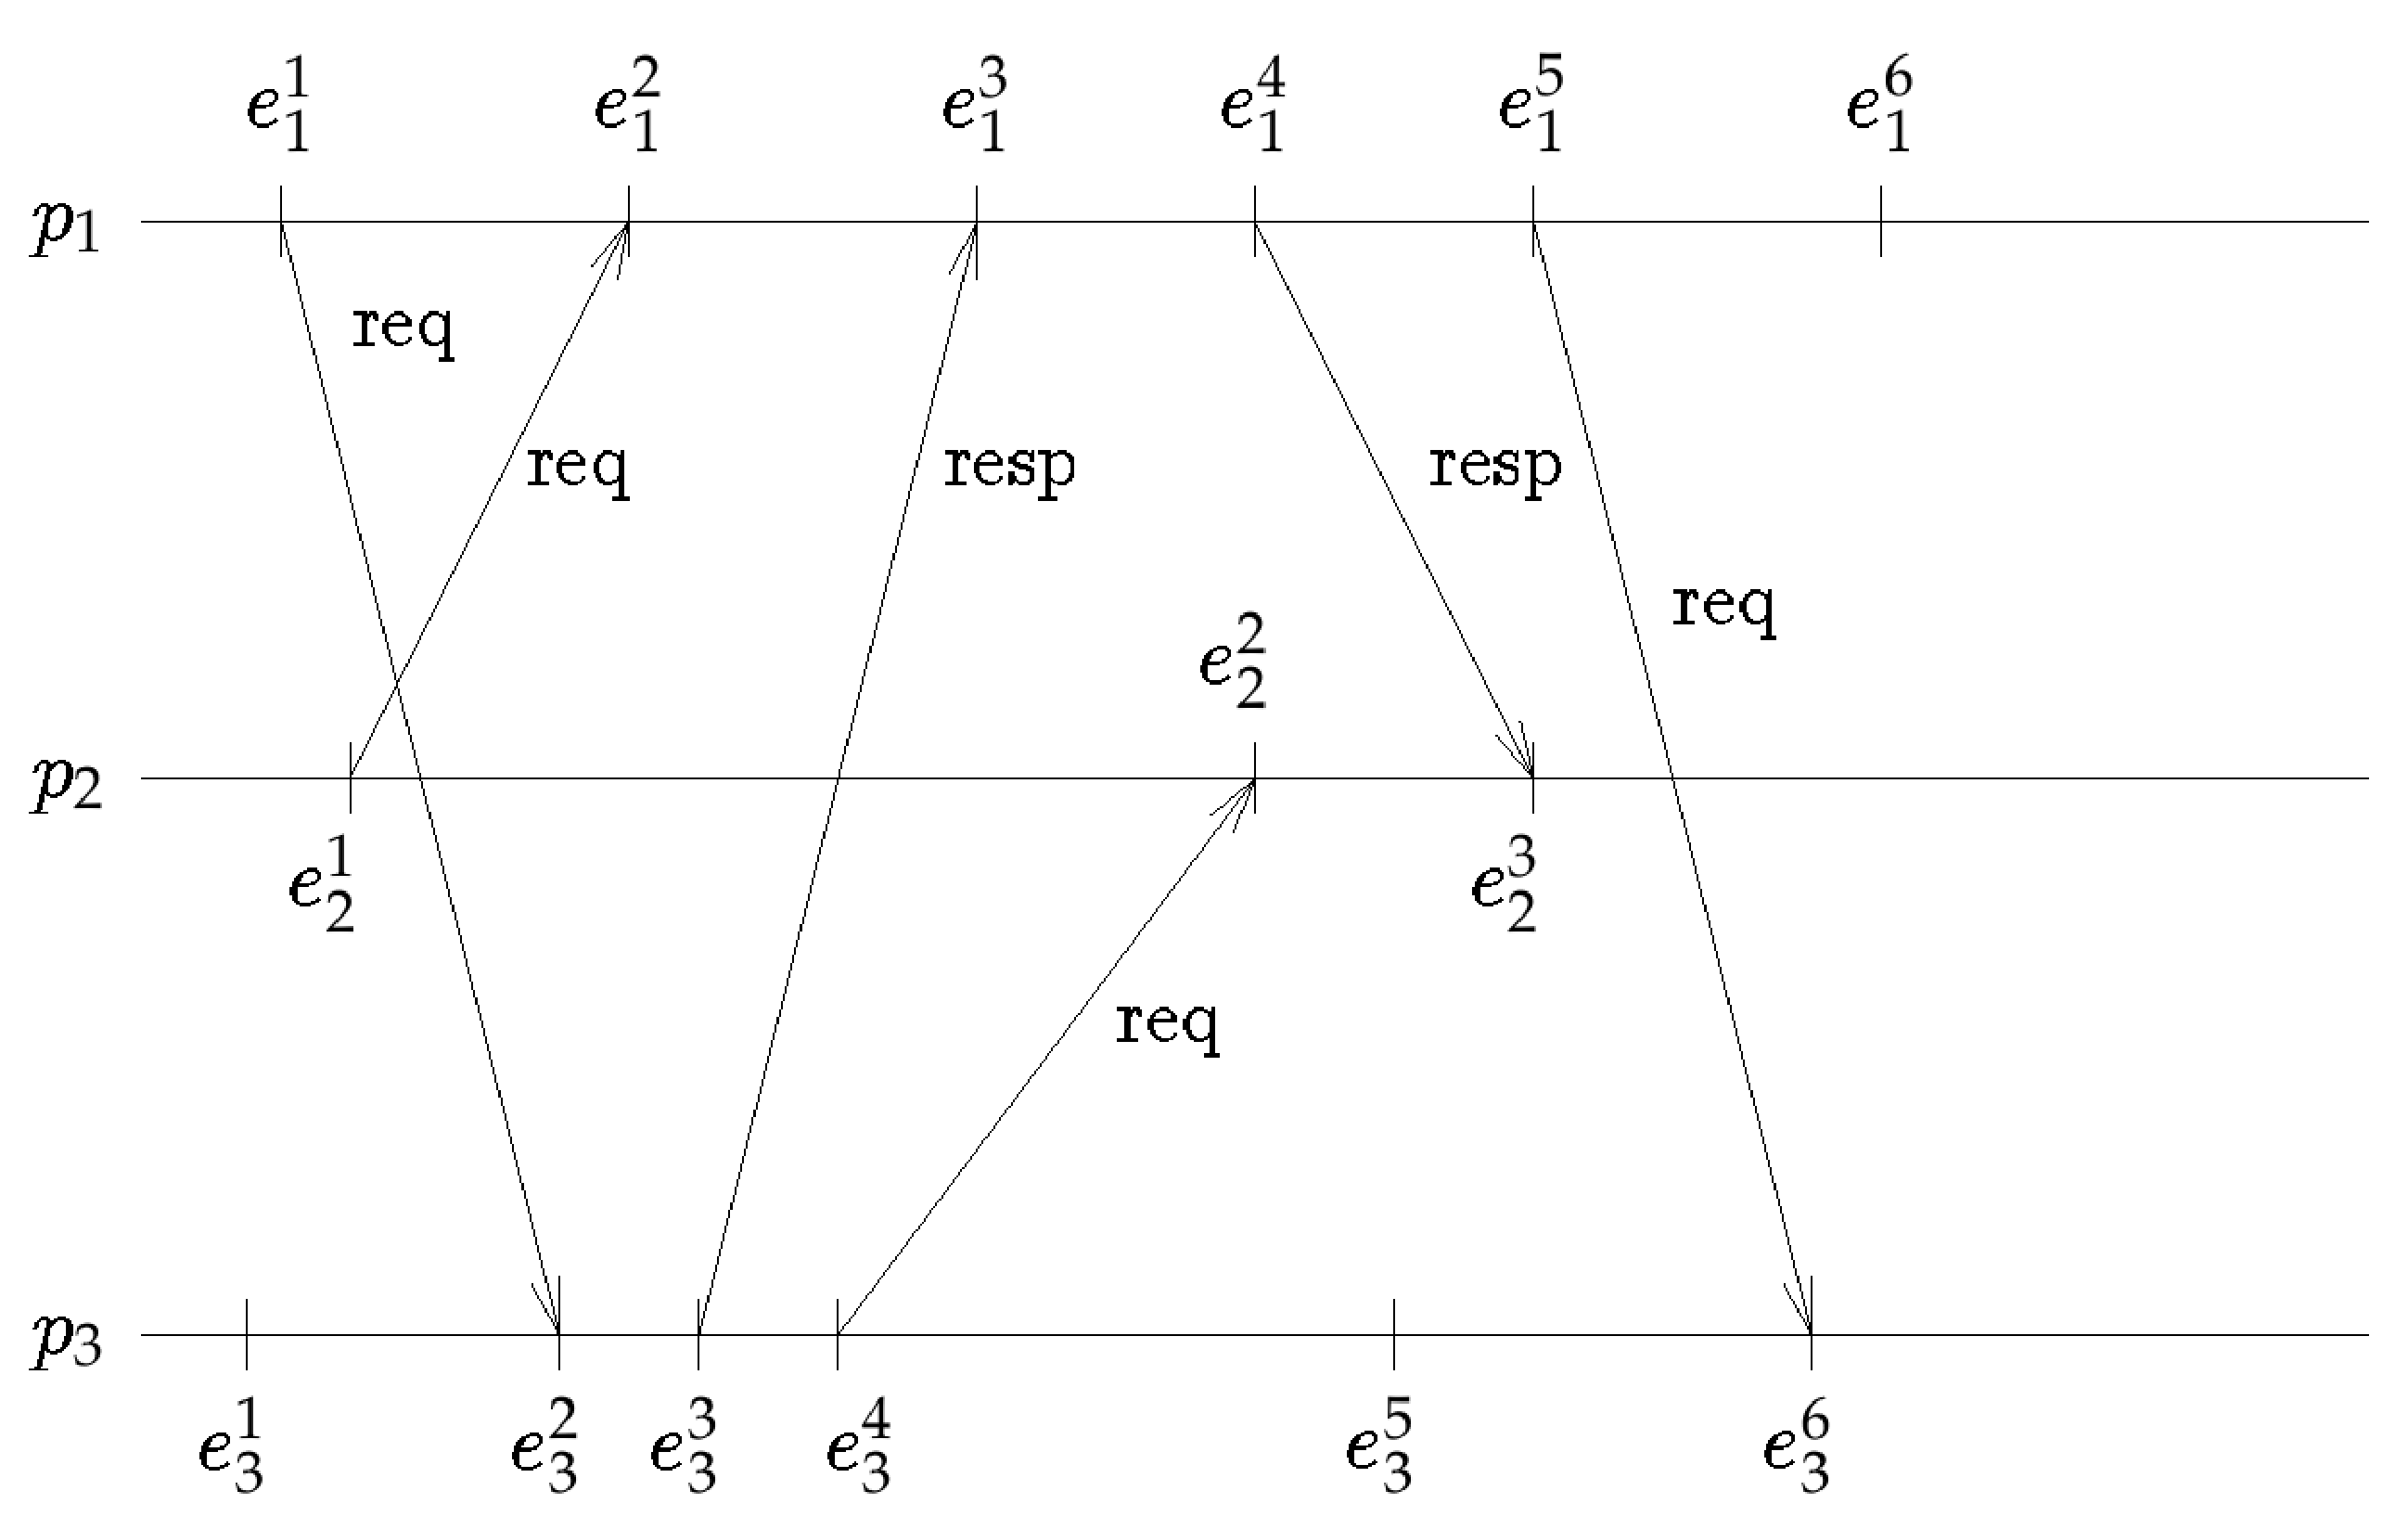
\includegraphics[width=10cm]{figs/02/figure-1}
\end{figure}

\end{frame}

\begin{frame}{Example -- Deadlock detection on a multi-tier system}

Processes in the previous figures use RPCs:
\BI
\item Client sends a \emph{request} for method execution; blocks.
\item Server receives \emph{request}.
\item Server executes method; may invoke other methods in other
servers, acting as a client.
\item Server sends \emph{reply} to client
\item Clients receives \emph{reply}; unblocks.
\EI

\bigskip
Such a system can deadlock, as RPCs are blocking. It is important to 
be able to detect when a deadlock occurs.

\end{frame}

\begin{frame}{Runs and consistent runs}
	
\begin{definition}[Run]
A \alert{run} of global computation is a total ordering $R$ that includes all the events
in the local histories and that is consistent with each of them.

\medskip
\BI
\item In other words, the events of $p_i$ appear in $R$ in the same order in which they appear in
$h_i$.
\item A run corresponds to the notion that events in a distributed computation
  actually occur in a total order
\item A distributed computation may correspond to many runs
\EI
\end{definition}

\begin{definition}[Consistent run]
A run $R$ is said to be \alert{consistent} if for all events $e$ and $e'$,
$e \rightarrow e'$ implies that $e$ appears before $e'$ in $R$.
\end{definition}
\end{frame}


\begin{frame}{Runs and consistent runs}

\BI
\item $e_1^1\,e_2^1\,e_3^1\,e_1^2\,e_2^2\,e_3^2\,e_3^1\,e_3^2\,e_3^3\,e_4^1\,e_4^3\,e_5^1\,e_5^3\,\,e_6^1\,e_6^3$ \ ?
\item $e_1^1\,e_2^1\,e_3^1\,e_1^2\,e_3^2\,e_3^3\,e_3^1\,e_4^1\,e_3^2\,e_4^3\,e_2^2\,e_5^1\,e_5^3\,\,e_6^1\,e_6^3$ \ ?
\EI

\begin{figure}
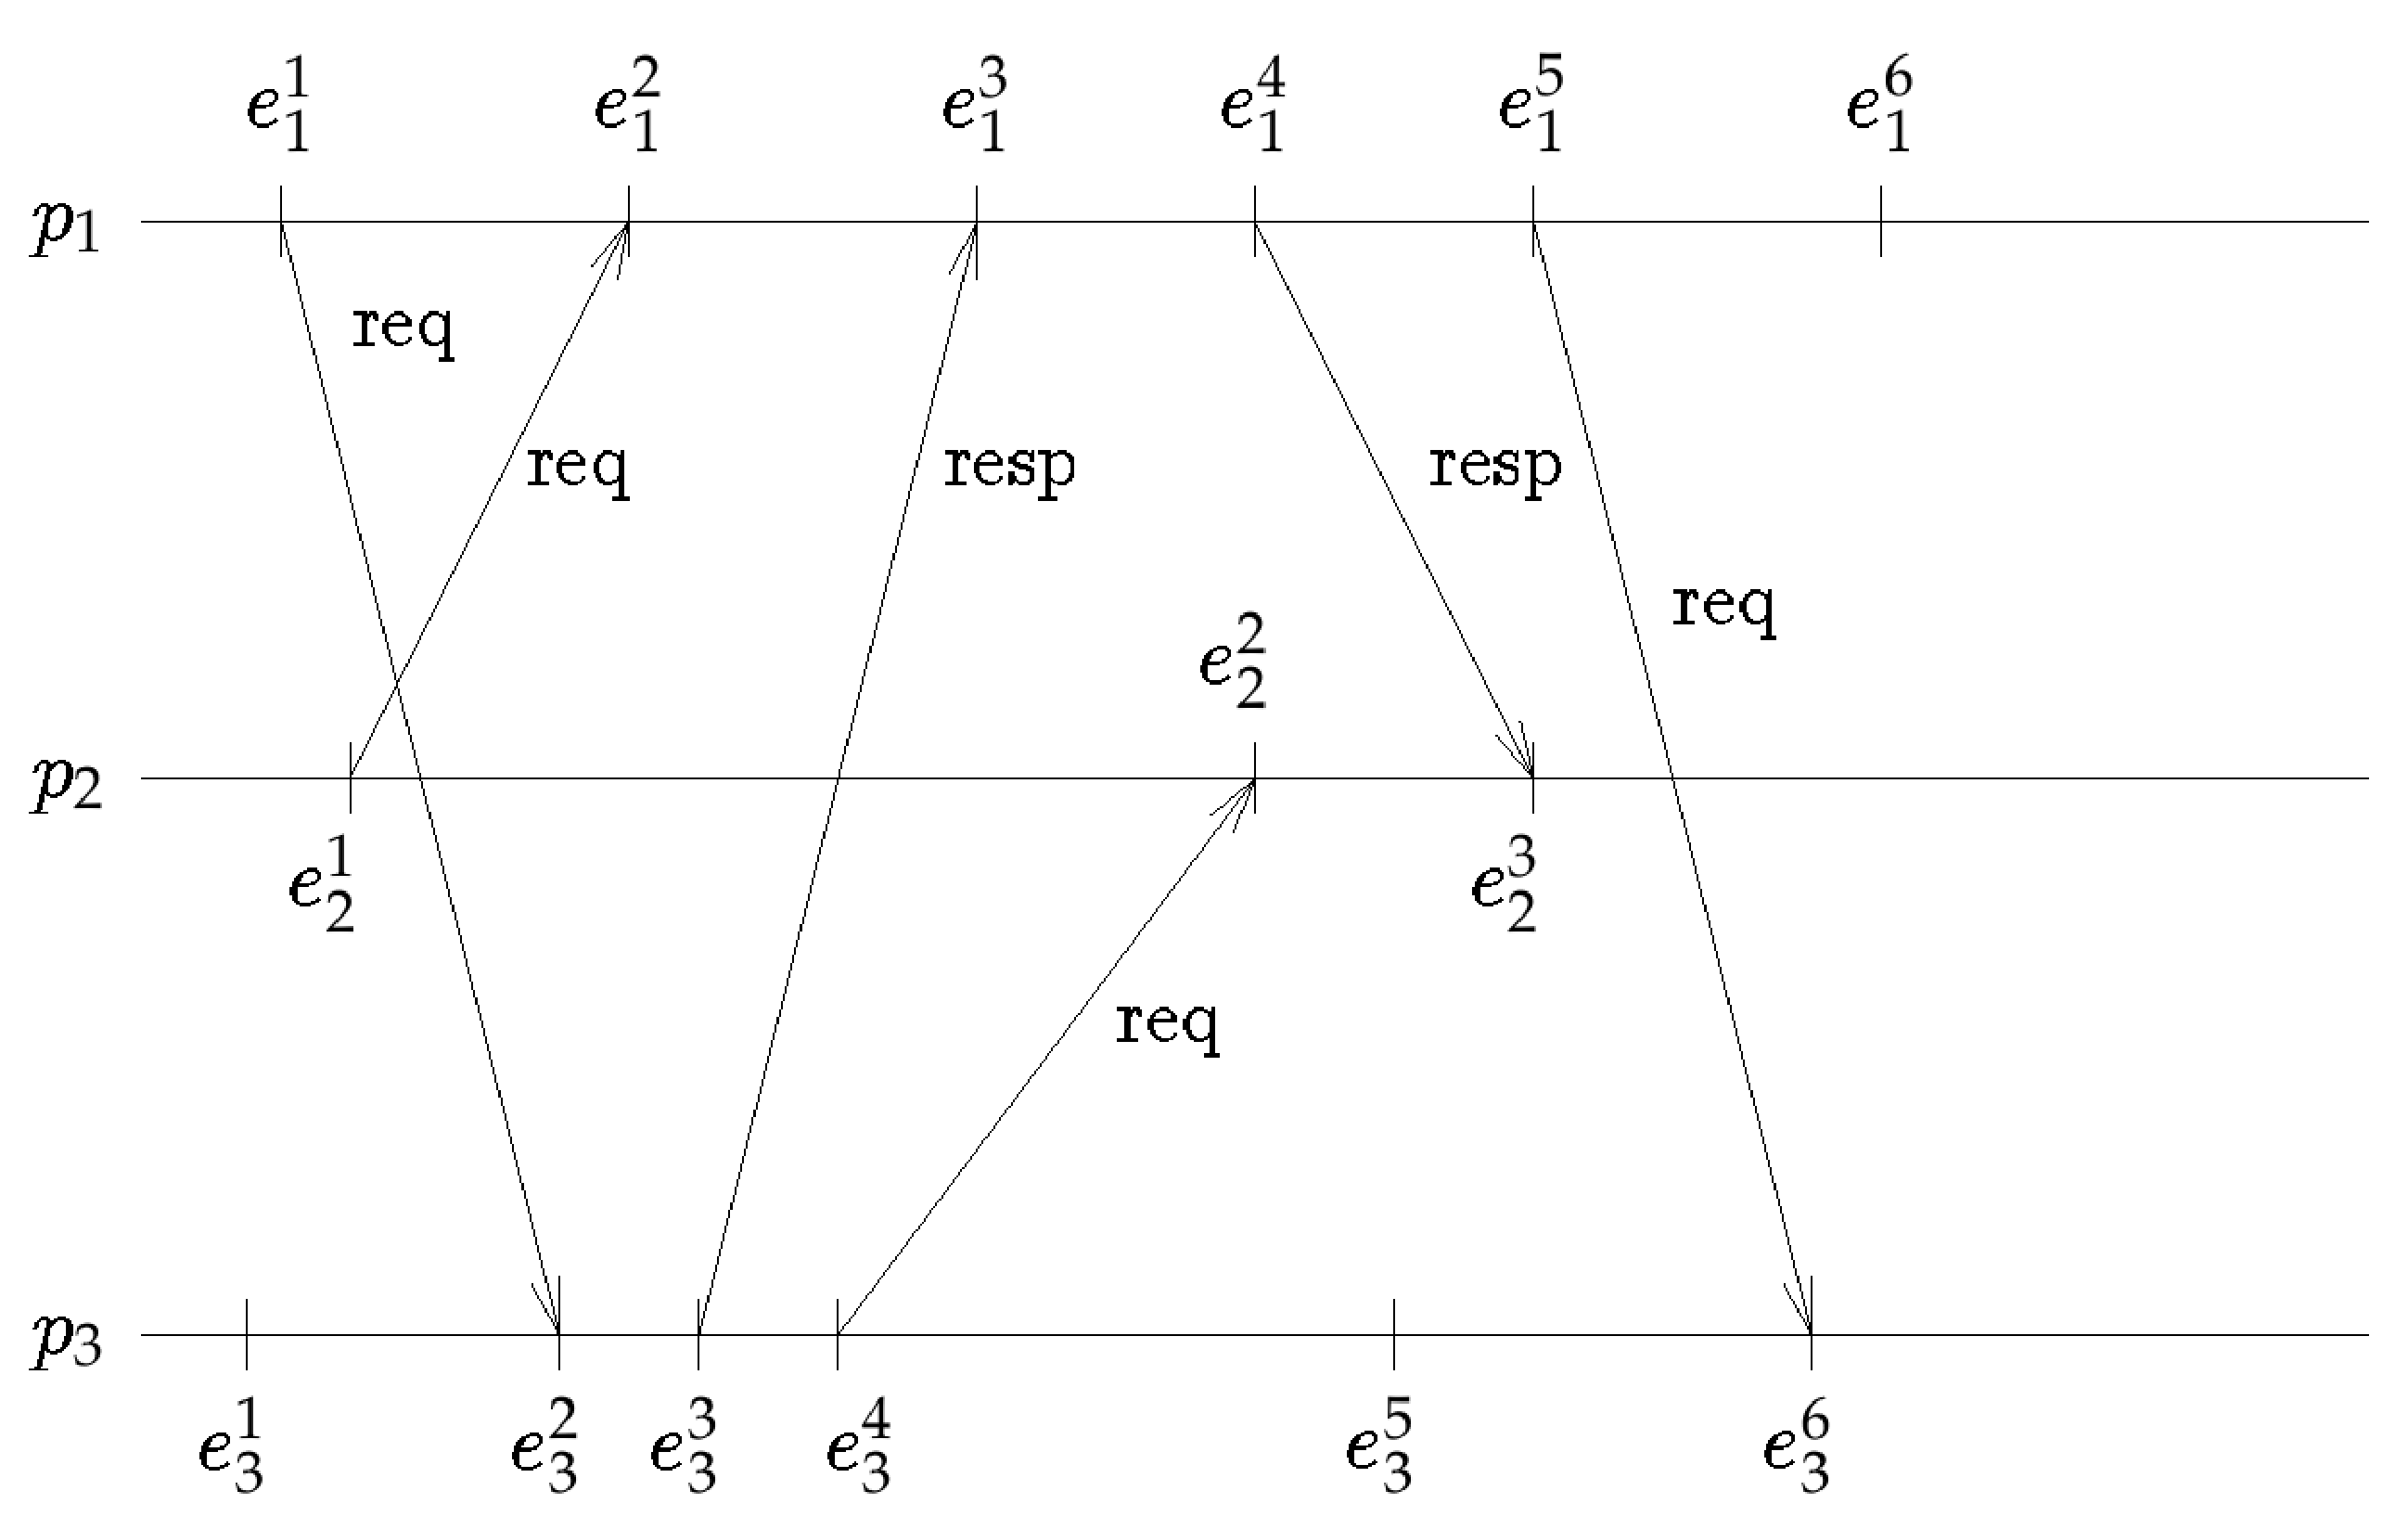
\includegraphics[width=9cm]{figs/02/figure-1}
\end{figure}

\end{frame}

\begin{frame}{Monitoring Distributed Computations}

\BIL
\item Assumptions: 
  \BI
  \item There is a single process $p_0$ called \alert{monitor} which
    is responsible for evaluating $\Phi$
  \item We assume that the monitor $p_0$ is distinct from the observed
    processes $p_1 \ldots p_n$ 
  \item Events executed on behalf of monitoring do not alter
    canonical enumeration of ``real'' events
  \EI
\item In general, observed processes send notifications about local events
  to the monitor, which builds an \alert{observation}. 
\EIL


\end{frame}

\begin{frame}{Observations}

\begin{definition}[Observation]
The sequence of events corresponding to the order in which notification
messages arrive at the monitor is called an \alert{observation}.
\end{definition}

\bigskip
Given the asynchronous nature of our distributed system, \emph{any}
permutation of a run $R$ is a possible observation of it.

\bigskip
\begin{definition}[Consistent observation]
An observation is \alert{consistent} if it corresponds to a consistent run.
\end{definition}

\end{frame}

\section{Real clocks vs logical clocks}

% \begin{frame}{The concept of causality}
% 
% \BIL
% % \item The concept of causality between events is fundamental to the design
% %   and analysis of distributed systems; e.g., it can be used to
% %   \BI
% %   \item maintain consistency in replicated databases
% %   \item design correct deadlock detection algorithms
% %   \item reconstruct a consistent state in checkpointing algorithms
% %   \EI
% \item The happen-before relation captures the concept of potential causality
% \item How can we use the concept of causality to design distributed
%   algorithms?
% % \item \alert{Causal order}: we want to deliver messages trying to avoid messages ``out-of-order''
% %   with respect to the happen-before relation
% \EIL
% 
% \end{frame}

\begin{frame}{How to obtain consistent observations}

\BIL
\item The happen-before relation captures the concept of potential causality
\item In the ``day-to-day'' life, causality/concurrency are tracked using
  physical time
  \BI
  \item We use loosely synchronized watches;
  \item Example: I have withdrawn money from an ATM in Trento at 13.00 on 17th May 2006,
    so I can prove that I've not withdrawn money on the same day at 13.20 in Paris
  \EI
\item In distributed computing systems:
  \BI
  \item the rate of occurrence of events is several magnitudes higher
  \item event execution time is several magnitudes smaller
  \EI
\item
  If physical clocks are not precisely synchronized, the
  causality/concurrence relations between events may not be accurately captured
\EIL

\end{frame}


\subsection{Logical clocks}

\begin{frame}{Logical clocks}
Instead of using physical clocks, which are impossible to synchronize,
we use logical clocks.
\BI
\item Every process has a \alert{logical clock} that is advanced using a
  set of rules
\item Its value is not required to have any particular relationship to any physical clock.
\item Every event is assigned a timestamp, taken from the logical clock
\item The causality relation between events can be generally inferred
  from their timestamps
\EI
\end{frame}

\begin{frame}{Logical clocks}

\begin{definition}[Logical clock]
A logical clock $LC$ is a function that maps an event $e$ from a distributed 
system execution to an element of a time domain $T$:
\[
  LC: H \rightarrow T
\]
\end{definition}

\begin{definition}[Clock Consistency]

\[ e \rightarrow e' \Rightarrow \LC(e) < \LC(e')  \]

\end{definition}

\begin{definition}[Strong Clock Consistency]

\[ e \rightarrow e' \Leftrightarrow \LC(e) < \LC(e')  \]

\end{definition}

\end{frame}


\subsection{Scalar logical clocks}

\begin{frame}{Scalar logical clocks}

\begin{definition}[Scalar logical clocks]
\BI
\item A Lamport's \alert{scalar} logical clock is a monotonically increasing software counter
\item Each process $p_i$ keeps its own logical clock $\LC_i$
\item The \alert{timestamp} of event $e$ executed by process $p_i$ is denoted $LC_i(e)$
\item Messages carry the \alert{timestamp} of their $\send$ event
\item Logical clocks are initialized to 0
\EI
\end{definition}

% \end{frame}
% 
% \begin{frame}{Scalar logical clocks: implementation}

\begin{block}{Update rule}
Whenever an event $e$ is executed by process $p_i$, its local logical clock is updated
as follows:
\[
\LC_i = \left\{ 
  \begin{array}{ll}
     LC_i + 1  & \mbox{If $e_i$ is an internal or $\send$ event} \\
     \max \{ LC_i, \TS(m) \} + 1 & \mbox{If $e_i = \receive(m)$}
  \end{array} 
\right.
\]
\end{block}
\end{frame}

\begin{frame}{Scalar logical clocks}

\begin{figure} 
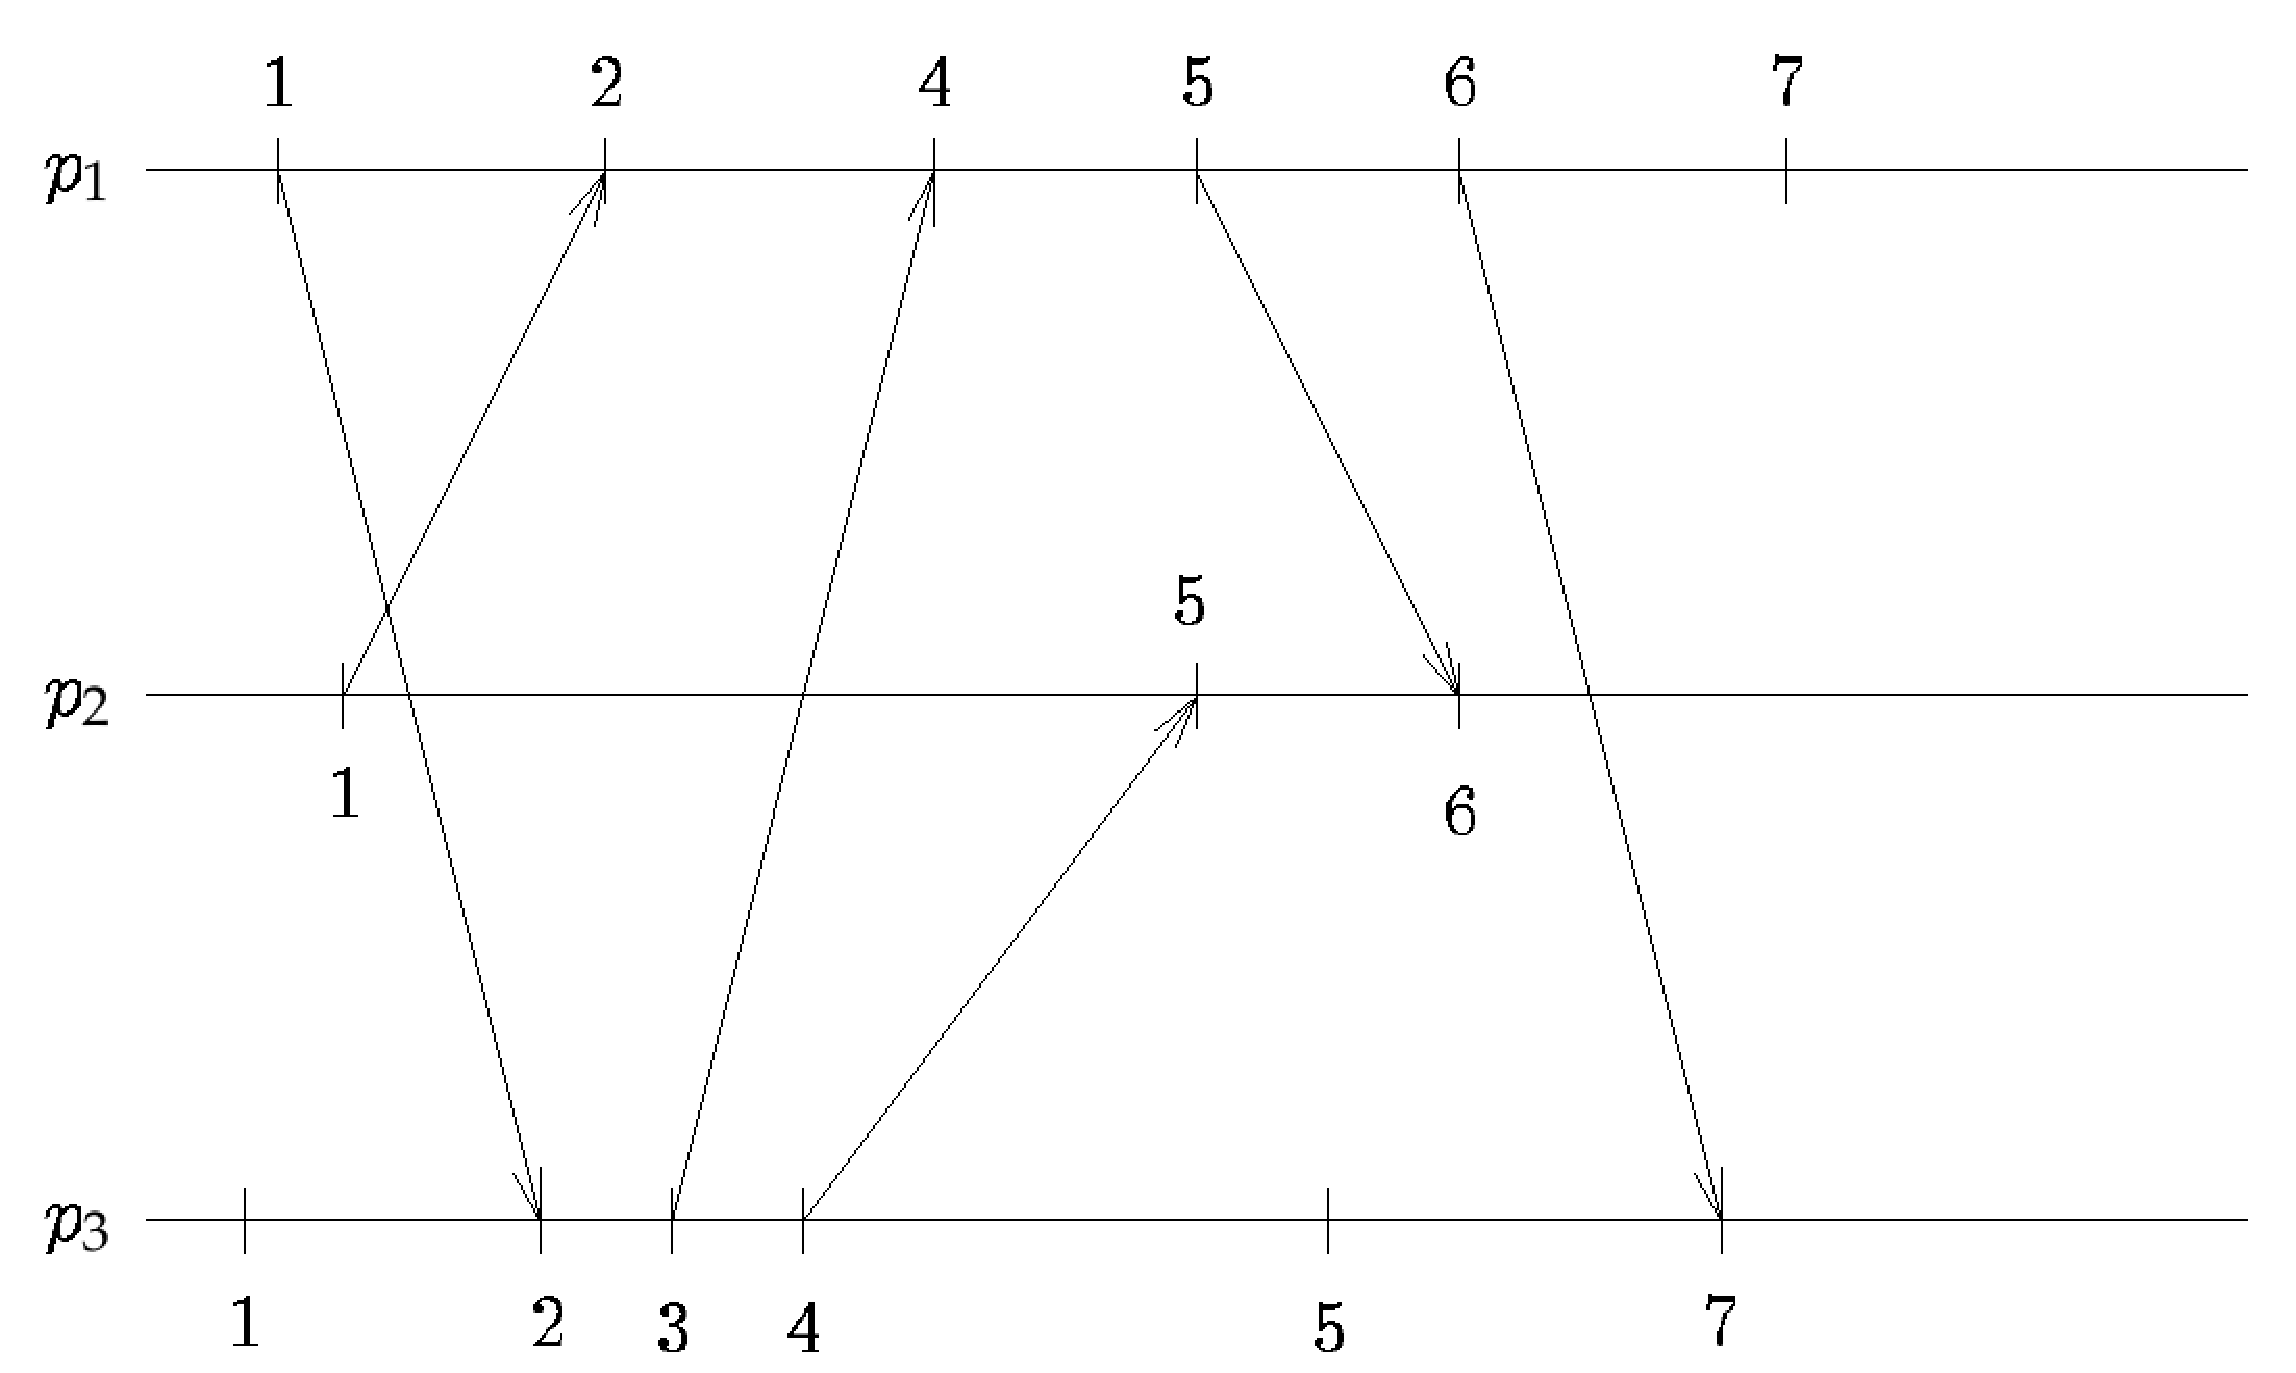
\includegraphics[width=10cm]{figs/02/figure-4}
\end{figure}

\end{frame}


\begin{frame}{Properties}

\begin{theorem}
Scalar logical clocks \emph{satisfy} Clock consistency, i.e.
\[
  e \rightarrow e' \Rightarrow LC(e) < LC(e')
\]
\end{theorem}

\pause
\begin{proof}
This immediately follows from the update rules of the clock.
\end{proof}


\note{
		
\emph{Total ordering}:
It is also possible to provide a total order for events, by sorting based
on the process identifier for events with the same timestamp. 
	
}


\end{frame}

\begin{frame}{Scalar logical clocks}

\begin{theorem}
Scalar logical clocks \emph{do not satisfy} Strong clock consistency, i.e.
\[
  LC(e) < LC(e') \not\Rightarrow e \rightarrow e' 
\]
\end{theorem}

\begin{figure} 
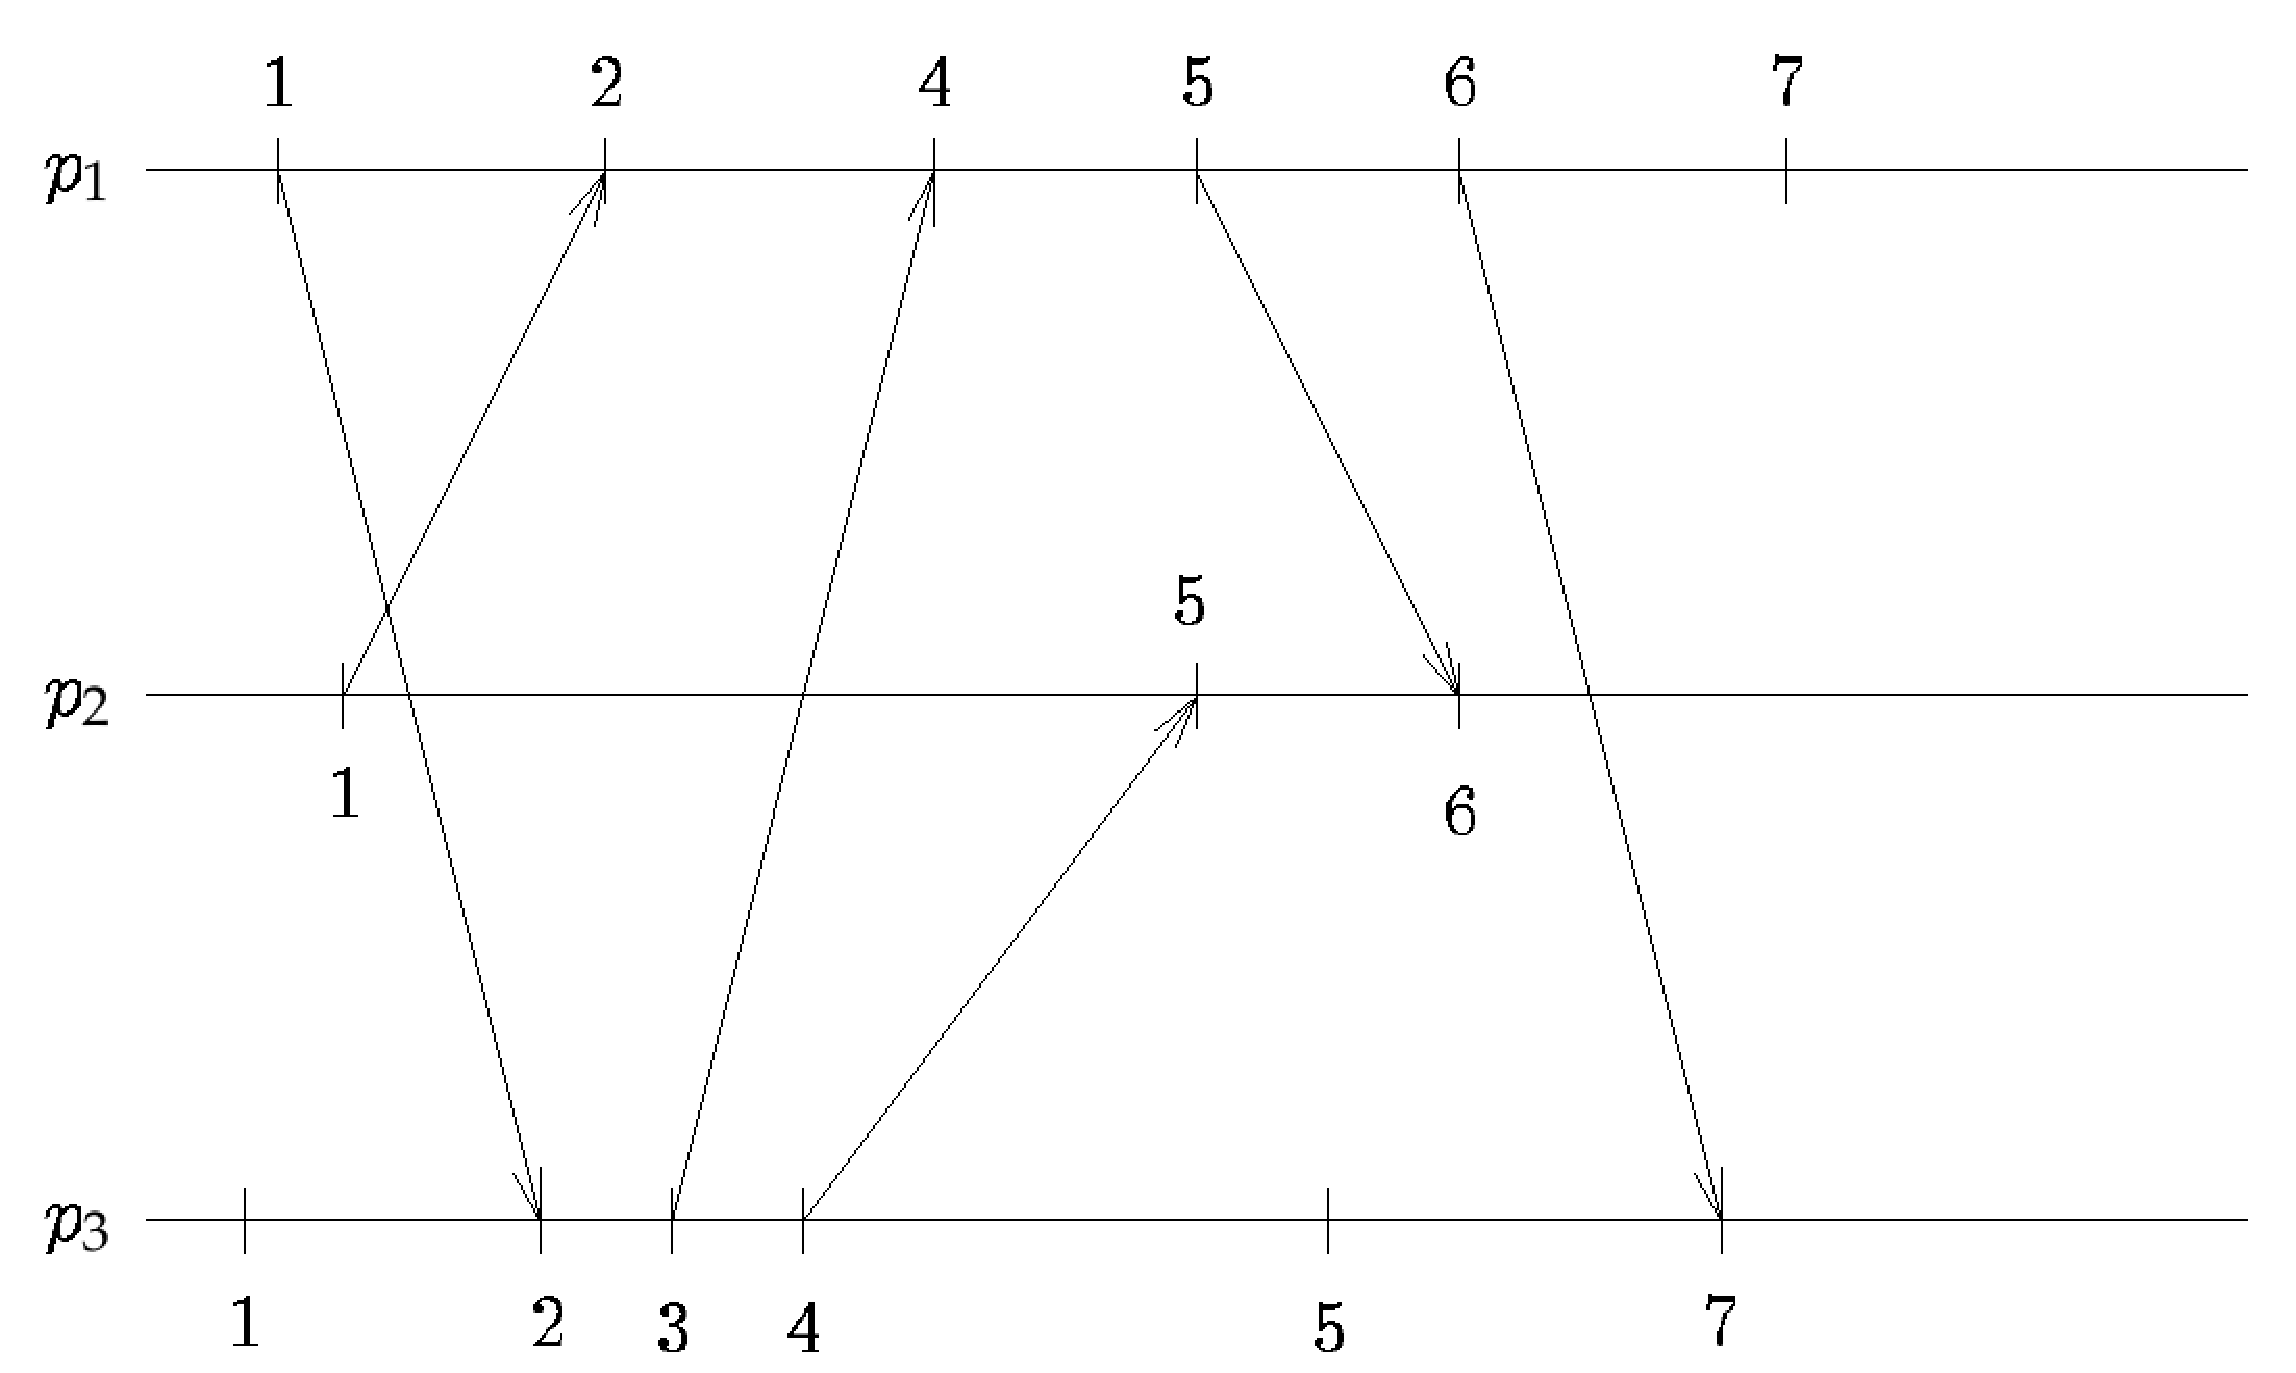
\includegraphics[width=8cm]{figs/02/figure-4}
\end{figure}

\note{

$LC(p_2^1) < LC(p_3^2)$, yet $p_2^1 \not\rightarrow p_3^2$

}


\end{frame}

% \begin{frame}{Further properties}
% 
% If a monitor is observing two events $e$ and $e'$, how can it discover whether
% there are further events executed after $e$ but before $e'$?
% 
% 
% \bigskip
% \begin{definition}[Gap detection for logical clocks]
% We say that a logical clock $\LC$ satisfies \alert{gap detection} if,
% given two events $e$ and $e'$ along with their clock values
% $\LC(e) < \LC(e')$, we are able determine whether some other event $e''$
% exists such that $\LC(e) < \LC(e'') < \LC(e')$.
% \end{definition}
% 
% \bigskip
% \structure{Problem:} \emph{Logical clocks do not guarantee gap detection}.
% 
% \end{frame}

\subsection{Vector logical clocks}

\begin{frame}{Causal histories clocks}

\begin{definition}[Causal History]
The \alert{causal history} of an event $e$ is the set of events that happen-before
$e$, plus $e$ itself.
\[
\theta(e) = \{ e' \in H ~|~ e' \rightarrow e \} \cup \{ e \}
\]
\end{definition}

\begin{theorem}
Causal histories \emph{satisfy} Strong clock consistency
\end{theorem}

\pause
\begin{proof}
\[
   \forall e \neq e': LC(e) < LC(e') \stackrel{def}{\Leftrightarrow} \theta(e) \subset \theta(e') \Leftrightarrow e \in \theta(e') \Leftrightarrow e \rightarrow e'
\]
\end{proof}

\end{frame}

% \begin{frame}{Causal delivery rule}
% 
% \begin{definition}[Causal History]
% The \alert{causal history} of an event $e$ is the set of events that happen-before
% $e$, plus $e$ itself.
% \[
% \theta(e) = \{ e' \in H ~|~ e' \rightarrow e \} \cup \{ e \}
% \]
% \end{definition}
% 
% \begin{theorem}
% Causal histories \emph{satisfy} Gap Detection
% \end{theorem}
% 
% \pause
% \begin{proof}
% Let $e, e'$ two events such that $e \neq e' \wedge \theta(e) \subset \theta(e')$. There are two
% cases:
% \BI
% \item if $\exists e'' \in \theta(e')-\theta(e)$, then $\theta(e) \subset \theta(e'') \subset \theta(e')$;
% \item otherwise, $\theta(e') = \theta(e) \cup e'$.
% \EI
% \end{proof}
% 
% 
% \end{frame}


\begin{frame}{Example}

\structure{Problem}: \\	
Causal histories tend to grow too much; they cannot be used as ``timestamps'' for messages.

\begin{figure} 
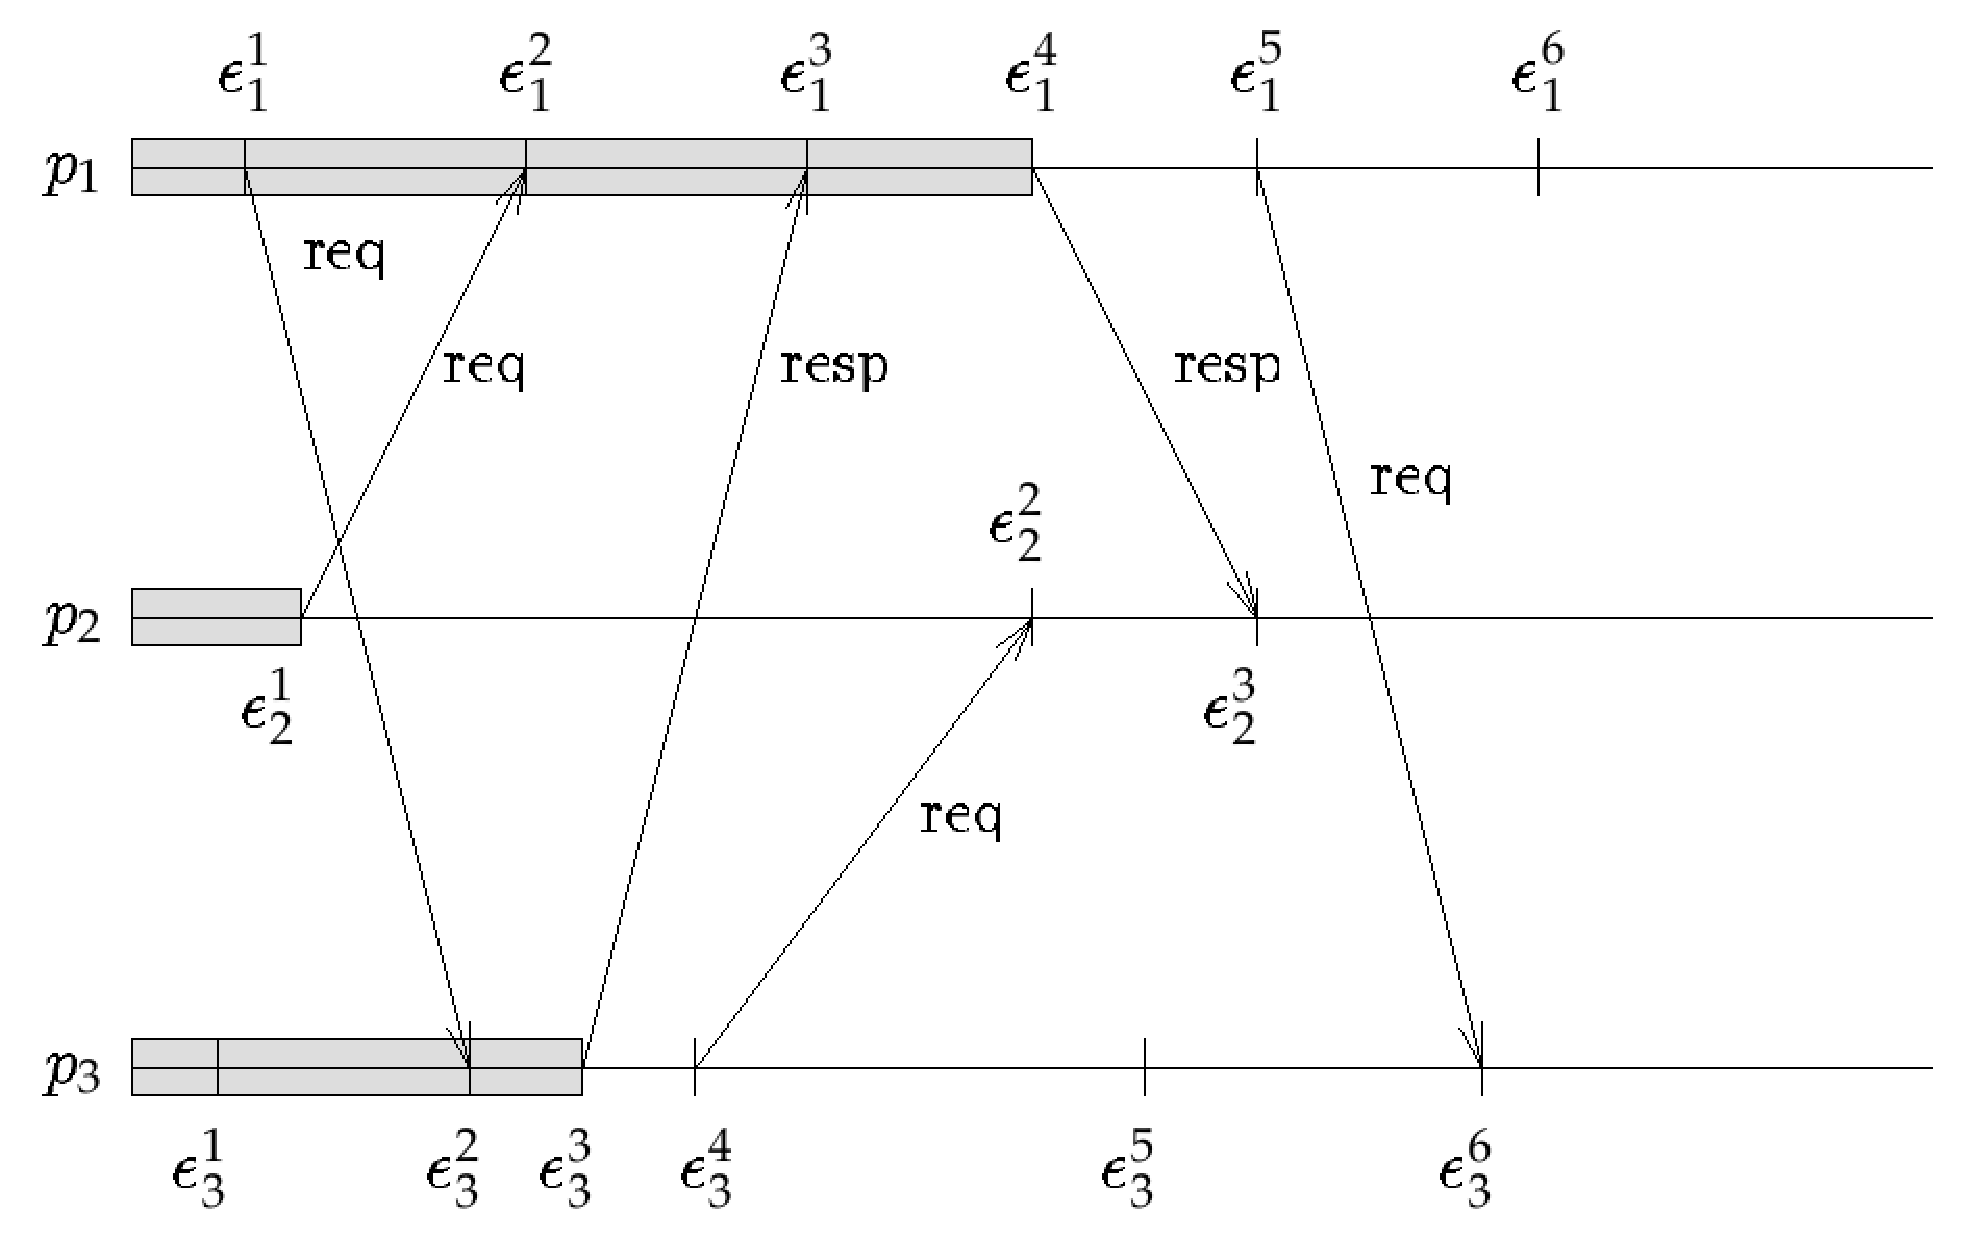
\includegraphics[width=9cm]{figs/02/figure-6}
\end{figure}
\end{frame}

\begin{frame}{Vector clocks}
\BI
\item Causal history projection: $\theta_i(e) = \theta(e) \cap h_i = h_i^{c_i}$
\item $\theta(e) = \theta_1(e) \cup \theta_2(e) \cup \ldots \cup \theta_n(e) = h_1^{c_1} \cup h_2^{c_2} \cup \ldots \cup h_n^{c_n}$
\item In other words, $\theta(e)$ is a cut, which happens to be consistent.
\item Cuts can be represented by their frontiers: $\theta(e) = (c_1, c_2, \ldots, c_n)$
\EI

\begin{definition}
The \alert{vector clock} associated to event $e$ is a $n$-dimensional vector $\VC(e)$ such that
\[
  \VC(e)[i] = c_i \qquad \mbox{where $\theta_i(e) = h_i^{c_i}$}
\]
\end{definition}


\end{frame}

\begin{frame}{Vector clocks: implementation}
\BI
\item Each process $p_i$ maintains a vector clock $\VC_i$, initially all zeroes;
\item When event $e_i$ is executed, $\VC_i$ assumes the value of $\VC(e_i)$;
\item If $e_i = \send(m)$, the timestamp of $m$ is $TS(m) = \VC(e_i)$;
\EI

\bigskip
\begin{block}{Update rule}
When event $e_i$ is executed by process $p_i$, $\VC_i$ is updated as follows:
\BI
  \item If $e_i$ is an internal or $\send$ event: 
\[
  \VC_i[i] = VC_i[i] + 1
\]
  \item If $e_i = \receive(m)$: \\
\[
  \begin{array}{ll}
    \VC_i[j] = \max \{ VC_i[j], TS(m)[j] \}  & \forall j \neq i \\
    \VC_i[i] = VC_[i] + 1
  \end{array} 
\]
\EI
\end{block}
\end{frame}

\begin{frame}{Example}
\begin{figure} 
\includegraphics[width=10cm]{figs/02/figure-7}
\end{figure}
\end{frame}

\begin{frame}{Properties of Vector clocks}

\begin{block}{``Less than'' relation for Vector clocks}
\[
  V < V' \Leftrightarrow (V \neq V') \wedge (\forall k: 1 \leq k \leq n: V[k] \leq V'[k])
\]
\end{block}

\begin{block}{Strong Clock Condition}
\[
  e \rightarrow e' \Leftrightarrow \VC(e) < VC(e') \Leftrightarrow \theta(e) \subset \theta(e')
\]
\end{block}

\begin{block}{Simple Strong Clock Condition}
\[
  e_i \rightarrow e_j \Leftrightarrow \VC(e_i)[i] \leq VC(e_j)[i]
\]
\end{block}

\end{frame}



\begin{frame}{Properties of Vector clocks}
	
\begin{definition}[Concurrent events]
Events $e_i$ and $e_j$ are {\em concurrent} (i.e. $e_i || e_j$) if and only if:
\[
   (VC(e_i)[i] > VC(e_j)[i]) \wedge (VC(e_j)[j] > VC(e_i)[j])
\]
\end{definition}

\bigskip
In other words, event $e_i$ does not happen-before $e_j$, and $e_j$ does not happen before
$e_i$.\\

\bigskip
\structure{Example}: ?

\end{frame}

\begin{frame}{Concurrent events}
\[
   (VC(e_i)[i] > VC(e_j)[i]) \wedge (VC(e_j)[j] > VC(e_i)[j])
\]

\begin{figure} 
\includegraphics[width=9cm]{figs/02/figure-7}
\end{figure}

\note{
Example of Concurrent Events:
Example: (3,1,3) and (1,2,4)
}

\end{frame}

\begin{frame}{Properties of vector clocks}
	
\begin{definition}[Pairwise Inconsistent]
Events $e_i$ and $e_j$ with $i \neq j$ are {\em pairwise inconsistent} if and only if
\[
   (VC(e_i)[i] < VC(e_j)[i]) \vee (VC(e_j)[j] < VC(e_i)[j])
\]
\end{definition}

\bigskip
In other words,  two events are pairwise inconsistent if they cannot belong to the frontier
of the same consistent cut. The formula characterize the fact that the cut include
a $\receive$ event without including a $\send$ event.\\

\bigskip
\structure{Example}: ?



\end{frame}


\begin{frame}{Pairwise inconsistent}
\[
   (VC(e_i)[i] < VC(e_j)[i]) \vee (VC(e_j)[j] < VC(e_i)[j])
\]

\begin{figure} 
\includegraphics[width=9cm]{figs/02/figure-7}
\end{figure}

\note{
Example of Pairwise Inconsistent Events:
Example: (3,1,3) and (1,0,2)

}

\end{frame}

\begin{frame}{Properties of Vector Clocks}
	
\begin{definition}[Consistent Cut]
A cut defined by $(c_1, \ldots, c_n)$ is \alert{consistent} if and only if:
\[
  \forall i,j \in [1 \ldots n]: \VC(e_i^{c_i})[i] \geq \VC(e_j^{c_j})[i])
\]
In other words, a cut is consistent if its frontier does not contain any
pairwise inconsistent pair of events.
\end{definition}

\end{frame}




\addtocontents{toc}{\newpage}

%%%%%%%%%%%%%%%%%%%%%%%%%%%%%%%%%%%%%%%%%%%%%%%%%%%%%%%%%%%%%%%%%%%%%

\section{Passive monitoring}

% \begin{frame}{Monitoring Distributed Computations}
% Two approaches:
%   \BI
%   \item Passive monitoring (receive notifications)
%   \item Proactive monitoring (ask to take a ``snapshot'')
%   \EI
% \end{frame}

\begin{frame}{A Passive Approach to GPE}

\structure{How it works}
\BI
\item At each (relevant) event, each process sends a \alert{notification} to the 
  monitor describing it local state
\item The monitor collects \alert{notifications} to reconstruct an observation of the global state.
\EI

\bigskip
\structure{An observation taken in this way can correspond to}:
\BI
\item A consistent run
\item A run which is not consistent
\item No run at all
\EI

\bigskip
Can you find example of the three cases?\\
Can you explain why this happen?
\end{frame}


\begin{frame}{Observations which are not runs}

\begin{block}{Problem} 
Observations may not correspond to a run because each \alert{notification} sent
by the process to the monitor may be delayed arbitrarily and thus 
arrive in any possible order
\end{block}

\pause
\bigskip
\begin{block}{Solution}
To adopt communication channels between the processes and the monitor that 
guarantee that messages are never re-ordered
\end{block}

\end{frame}

\begin{frame}{Message ordering}
\begin{definition}[FIFO  Order]
Two messages sent by $p_i$ to $p_j$ must be delivered in the
same order in which they were sent:
\[
\forall m,m': \send_i(m) \rightarrow \send_i(m') \Rightarrow \deliver_j(m) \rightarrow \deliver_j(m')
\]
\end{definition}

\bigskip
Uh? What is ``deliver''?

\end{frame}

\begin{frame}{Delivery Rules}

\structure{How to order messages?}
\BI
\item To be ordered, each message $m$ carries a \alert{timestamp} $\TS(m)$ 
  containing ``ordering'' information
\item The act of providing the process with a message in the desired order
  is called \alert{delivery}; the event $\deliver(m)$ is thus distinct from
  $\receive(m)$.
\item The rule describing which messages can be delivered among those 
  received is called \alert{delivery rule}
\EI

\end{frame}


\begin{frame}{FIFO Order - Implementation} 
	
\BI
\item Each process maintains a \alert{local sequence number} incremented at
  each notification sent
\item The timestamp of a notification message corresponds to the local sequence number
  of the sender at the time of sending
\EI

\begin{definition}[FIFO Delivery Rule]~\\
  If the last notification delivered by $p_0$ from $p_j$ has timestamp
  $s$, $p_0$ may deliver ``any'' message $m$ received from $p_j$ with $\TS(m)=s+1$.
\end{definition}

\end{frame}


%%% TODO: Add figure

\begin{frame}{Observations which are not consistent runs}

\begin{block}{Problem} 
If we use FIFO order between all processes and $p_0$, all the observations taken by $p_0$ will be \emph{runs};
but there is no guarantee that they are \emph{consistent runs}.
\end{block}

\pause
\bigskip
\begin{block}{Solution}
To adopt communication channels that guarantee that notification arrives
in an order that respects the happen-before relation.
\end{block}

\end{frame}

\begin{frame}{Message ordering}

\begin{definition}[Causal Order]
Two messages sent by $p_i$ and $p_j$ to $p_k$ must be delivered following
the happen-before relation:
\[
\forall m,m': \send_i(m) \rightarrow \send_j(m') \Rightarrow \deliver_k(m) \rightarrow \deliver_k(m')
\]
\end{definition}

\bigskip
\begin{block}{Question}
 FIFO order among all channels...\\
 Is it sufficient to obtain Causal delivery?
\end{block}

\end{frame}


\begin{frame}{Example}

\note{
\BIL
\item Given that each communication channels is associated with just one message,
this distributed system satisfies the FIFO order.

\item However, it does not satisfy Causal order: the deliver of message $m'$ should 
be delivered after message $m$, because the send event of $m$ is potentially
caused by $m'$.

\item Silly example: $p_1$ sends an invitation for a party to $p_2$ and  $p_3$ by SMS; $p_2$
sends a message to $p_3$ saying “Are you going to participate to the party of
$p_1$?” $p_3$ gets offended because it has not been invited.
\EIL

}

\begin{figure} 
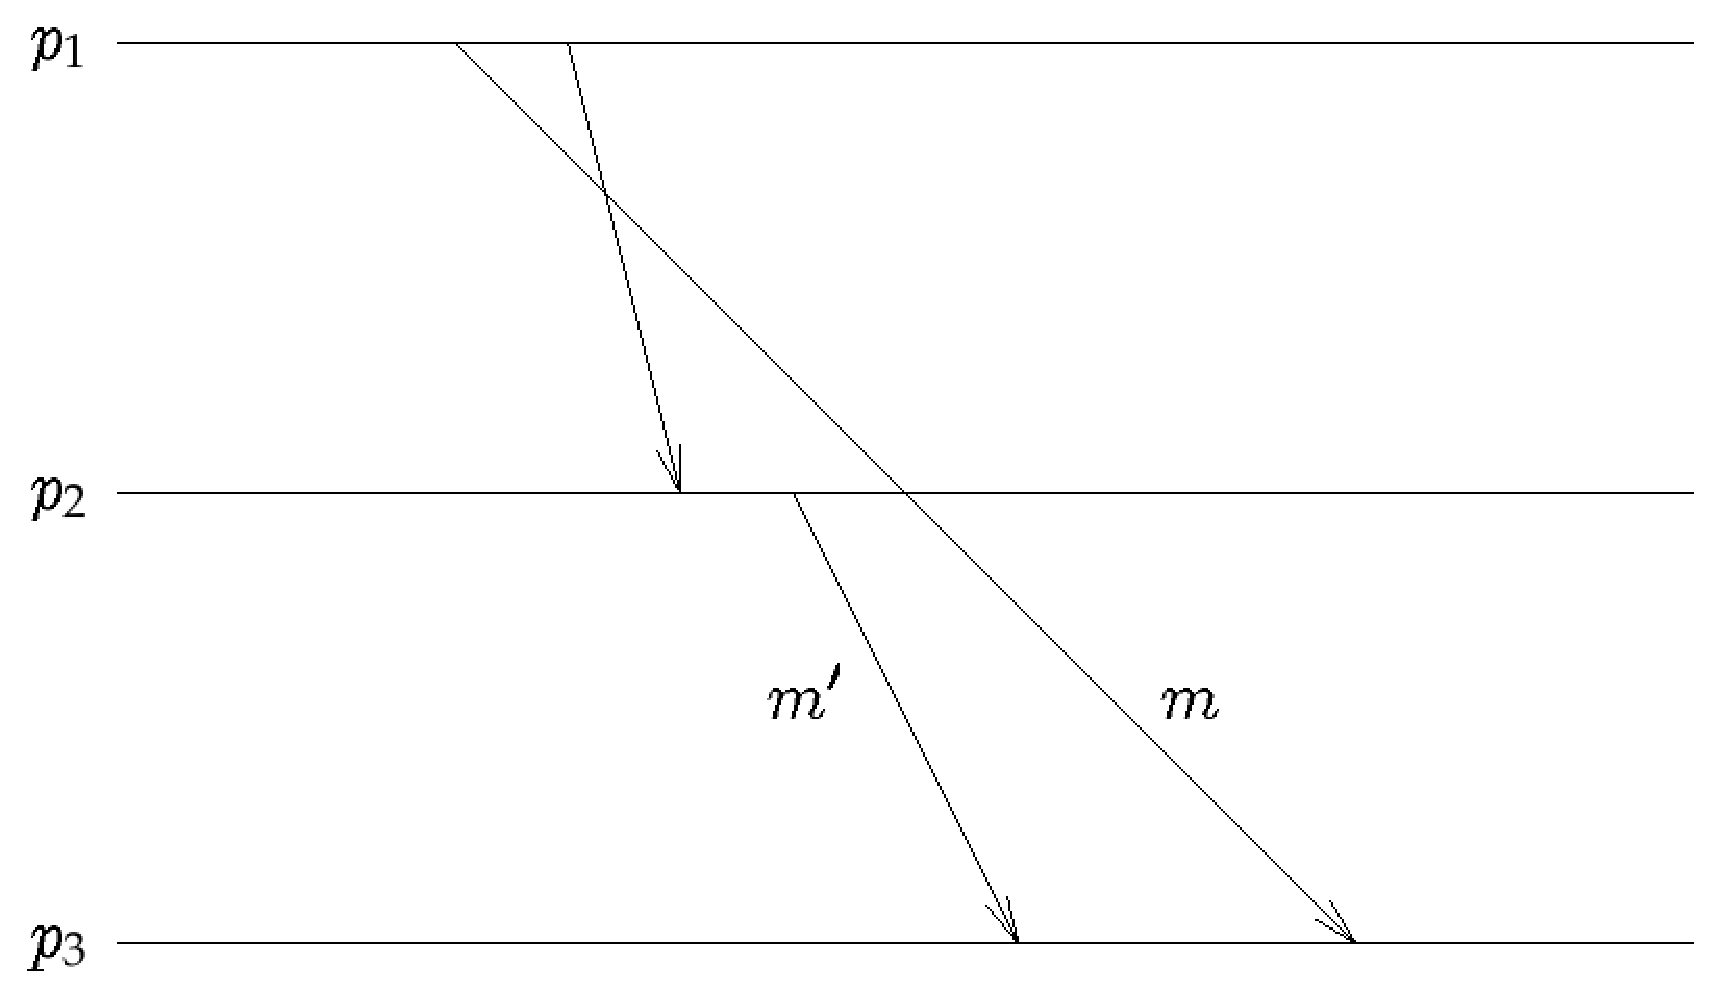
\includegraphics[width=11cm]{figs/02/figure-5}
\end{figure}

\end{frame}

\begin{frame}{Causal delivery and consistent observations}

\begin{theorem}
If $p_0$ uses a delivery rule satisfying Causal Order, then all of its
observations will be consistent.
\end{theorem}

\bigskip
\begin{proof}
Definition of Causal Order $\equiv$ definition of a consistent observation
\end{proof}

\bigskip
Next, we will show three methods to implement a causal delivery rule



\note{
\BI
\item Suppose, by contradiction, that the monitor obtains an observation which is not consistent. 
\item This means that an event $e'$ appears before $e$ in the observation, but $e \rightarrow e'$. 
\item By the strong clock condition, because $e \rightarrow e'$, this means that $\VC(e) < \VC(e')$. 
\item By definition of Causal Order, this means that $e'$ cannot appear \\
before $e$, a contradiction.
\EI
}


\end{frame}


\subsection{Passive monitoring, v.1}

\begin{frame}{Passive monitoring with real-time}

\structure{Initial assumptions}
\BI
\item All processes have access to a real-time clock $\RC$
\item Let $\RC(e)$ be the real-time at which $e$ is executed
\item All messages are delivered within a time $\delta$
\item The timestamp of message $m$ sent by an event $e = \send(m)$
  is $\TS(m) = \RC(e)$.
\EI
\begin{definition}[DR1: Real-time delivery rule]
At any time, delivery all received notification messages $m$ 
in increasing timestamp order.
\end{definition}
\begin{overprint}
\onslide<1|handout:1>
\begin{theorem}
Observation $O$ constructed by $p_0$ using DR1 is guaranteed to be
consistent (?)
\end{theorem}
\onslide<2|handout:2>
\begin{theorem}
\sout{
Observation $O$ constructed by $p_0$ using DR1 is guaranteed to be
consistent
}
\end{theorem}
\end{overprint}


\end{frame}

\begin{frame}{Stability of messages}

\begin{definition}[Stability] A notification message $m$ received by $p_0$ is \alert{stable at $p_0$} if no message
$m'$ with $\TS(m') < \TS(m)$ can be received in the future by $p_0$
\end{definition}


\begin{definition}[DR1: Real-time delivery rule]
At time $t$, delivery all received notification messages $m$ \emph{such that
$\TS(m) \leq t-\delta$} in increasing timestamp order.
\end{definition}
\medskip
\begin{theorem}
Observation $O$ constructed by $p_0$ using DR1 is guaranteed to be
consistent
\end{theorem}


\end{frame}


\begin{frame}{Proof}

\begin{block}{Safety: Clock Condition for $\RC$} 
\[
  e \rightarrow e' \Rightarrow \RC(e) < \RC(e') 
\]
Note that $\RC(e) < \RC(e') \not\Rightarrow e \rightarrow e'$, but 
this rule is sufficient to obtain consistent observations, as
two notifications $e \rightarrow e'$ are never delivered in the incorrect
order.
\end{block}

\medskip
\begin{block}{Liveness: Stability}
At time $t$, any message sent by time $t-\delta$ is stable.
\end{block}

\medskip
Note that real-time clocks do not support stability; it is the
maximum delay of messages that enables it.
\end{frame}

\subsection{Passive monitoring, v.2}


\begin{frame}{Passive monitoring with logical clocks}

\structure{Initial assumptions}
\BI
\item All processes have access to a logical clock $\LC$; \\
  let $\LC(e)$ be the logical clock at which $e$ is executed
\item The timestamp of message $m$ sent through an event $e = \send(m)$
  is $\TS(m) = \mathit{LC}(e)$
\EI

\begin{definition}[DR2: Deliver Rule for $\LC$]
Deliver all received messages that are stable at $p_0$ in increasing timestamp order
\end{definition}

\end{frame}


\begin{frame}{Passive monitoring with logical clocks}

\begin{block}{Safety: Clock Condition for $\LC$} 
\[
e \rightarrow e' \Rightarrow \LC(e) < \LC(e')
\] 
Note that $\LC(e) < \LC(e') \not\Rightarrow e \rightarrow e'$, but 
this rule is sufficient to obtain consistent observations, as
two events $e \rightarrow e'$ are never ordered incorrectly
\end{block}

\end{frame}

\begin{frame}{Passive monitoring with logical clocks}

\begin{block}{Liveness: Stability} We need a way to reproduce the concept
	of $\delta$ in an asynchronous system, otherwise no notification message
	will be ever delivered.
\end{block}

\begin{block}{Solution}
\BIL
\item Each process communicates with $p_0$ using FIFO delivery
\item When $p_0$ receives a message from $p_i$ describing an event $e$ 
with timestamp $\TS(e)$, it is sure that it will never receive a message
from $p_i$ describing an event $e'$ with $TS(e') \leq TS(e)$
\item Stability of message $m$ at $p_0$ can be guaranteed when $p_0$ has
received at least one message from all other processes with a timestamp
greater or equal than $\TS(m)$
\EIL
\end{block}

\end{frame}

\begin{frame}{Problems of Logical Clocks}
\BI
\item They add unnecessary delays to observations
\item They require a constant flux of messages/events from all processes
\EI

\begin{figure}
	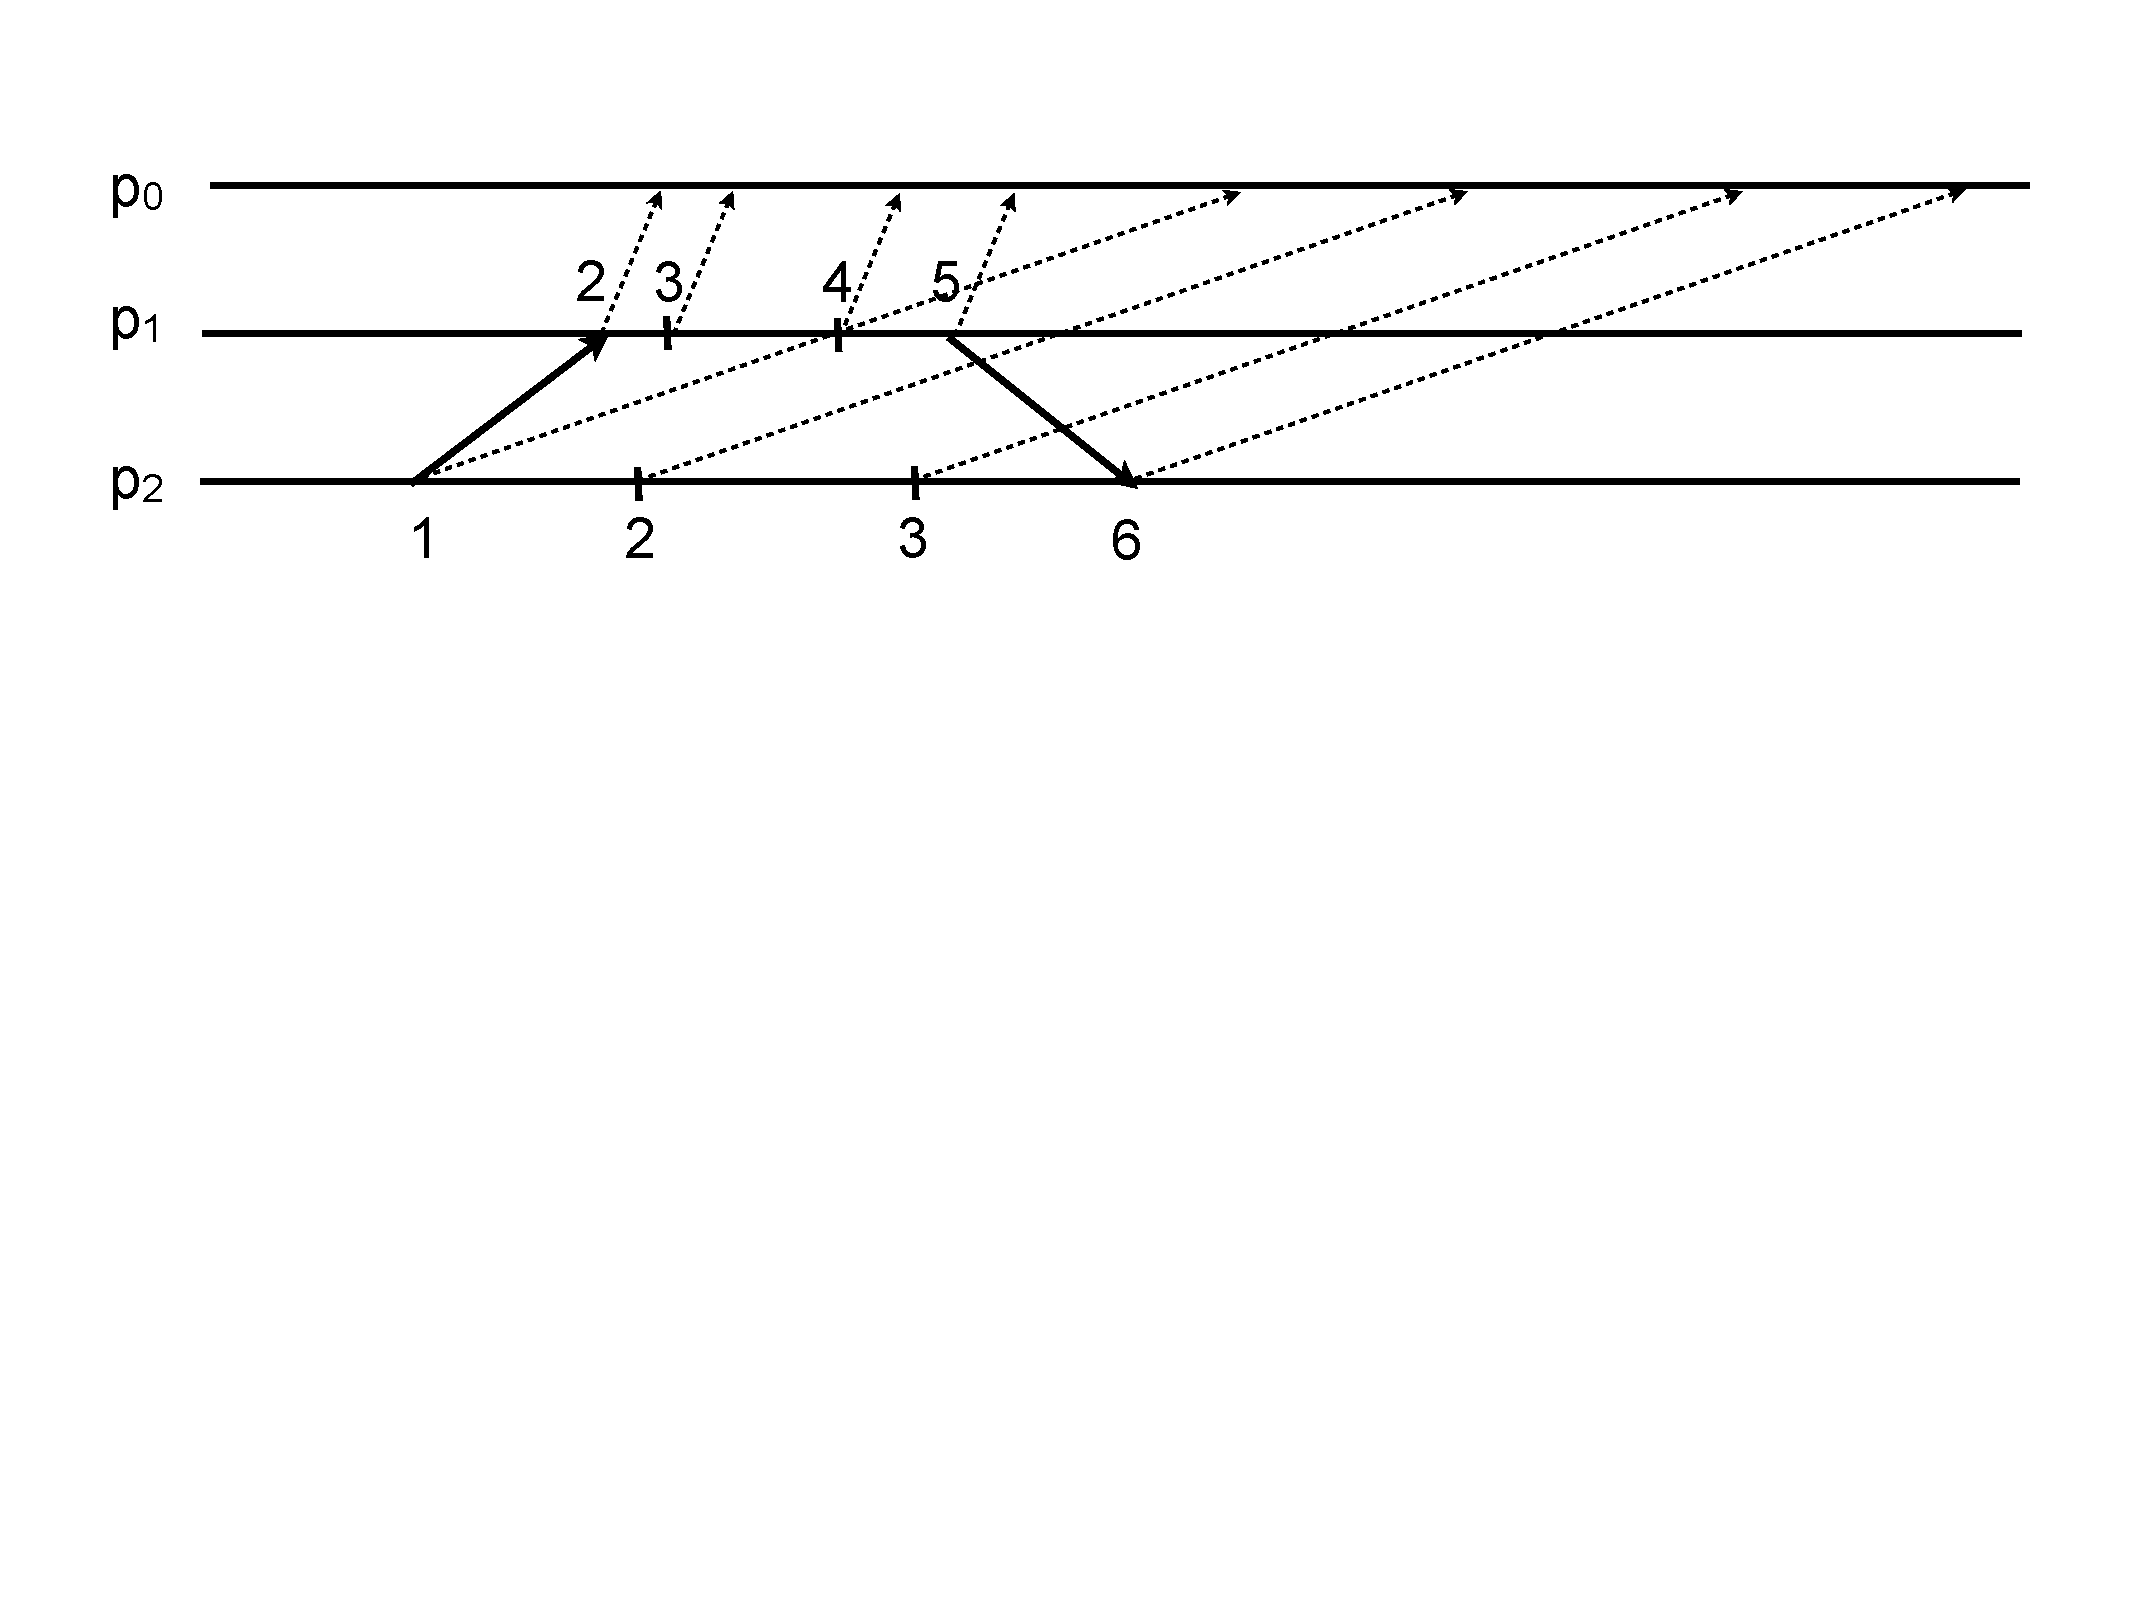
\includegraphics[width=12cm]{figs/03/figura.pdf}
\end{figure}

\end{frame}

% \begin{frame}{Limitations of Logical Clocks}
% 
% \structure{Clock Condition is not sufficient}
% \BI
% \item Logical Clocks guarantee that $e \rightarrow e' \Rightarrow LC(e) < LC(e')$;
% \item This means that $LC(e) < LC(e') \Rightarrow e' \not\rightarrow e$;
% \item This means that if we receive $e'$ before $e$, we must delay $e'$, even if we 
%   could predict the timestamps of all events yet to be received
% \item Smaller timestamps: may be concurrent or may have happened-before
% \EI
% 
% We need a clock mechanism $C$ satisfying:
% 
% \alert{Strong Clock Condition}: $e \rightarrow e' \Leftrightarrow C(e) < C(e')$;
%  
% 
% \end{frame}

\subsection{Passive monitoring, v.3}





\begin{frame}{Passive Monitoring with Vector Clocks}
	
\structure{Variables maintained at $p_0$}

\BI
\item $\cal M$: the set of notification messages received but not yet delivered by $p_0$
\item an array $D$, initialized to 0's, such that $D[k]$ contains $TS(m)[k]$ where $m$
  is the last notification message delivered by $p_0$ from process $p_k$.
\EI

\bigskip
\structure{When a notification message is deliverable by $p_0$?}

A notification message $m \in \cal M$ from process $p_j$ is deliverable as soon as $p_0$
can verify that there is no other notification message $m'$ (neither in $\cal M$ nor in the 
channels) such that $\send(m') \rightarrow \send(m)$.

\end{frame}


\begin{frame}{Implementing Causal Delivery with Vector Clocks}

\BI
\item $m \in \cal M$: a notification message sent by $p_j$ to $p_0$
\item $m'$: the last notification message delivered from process $p_k$, $k \neq j$
\EI

\bigskip
\begin{definition}[Weak Gap Detection]
If $\TS(m')[k] < \TS(m)[k]$ for some $k \neq j$, then there exists event $\send_k(m'')$ such that
\[
  \send_k(m') \rightarrow \send_k(m'') \rightarrow \send_j(m)
\]
\end{definition}

\bigskip
\end{frame}

% \begin{frame}{Weak Gap Detection}
% \[
%    \VC(e_i)[k] < \VC(e_j)[k] \wedge k \neq j \Rightarrow e_k \not\rightarrow e_i \wedge e_k \rightarrow e_j
% \]
% \begin{figure} 
% \includegraphics[width=9cm]{figs/03/figure-7}
% \end{figure}
% \end{frame}


\begin{frame}{Implementing Causal Delivery with Vector Clocks}

\structure{Two conditions to be verified}:

\BIL

\item There is no earlier message from $p_j$ that has not been delivered yet.
\begin{overprint}
\onslide<1|handout:0>
 \alert{How can we express this condition?}
\onslide<2-3|handout:1>
  \alert{Causal Delivery Rule, Part 1}  $D[j] == \TS(m)[j] -1$
\end{overprint}

\item $\forall k \neq j$, let $m'$ be the last message from $p_k$ delivered by $p_0$ ($D[k] = \TS(m')[k]$); 
we must be sure that no message $m''$ from $p_k$ exists such that:
$
\send_k(m') \rightarrow \send_k(m'') \rightarrow \send_j(m)
$
\begin{overprint}
\onslide<1-2|handout:0>
  \alert{How can we express this condition?}
\onslide<3|handout:1>
\alert{Causal Delivery Rule, Part 2}: $\forall k \neq j: D[k] \geq \TS(m)[k]$\\
It follows from Weak Gap Detection
\end{overprint}

\EIL

\end{frame}

\begin{frame}{Example}
\begin{figure} 
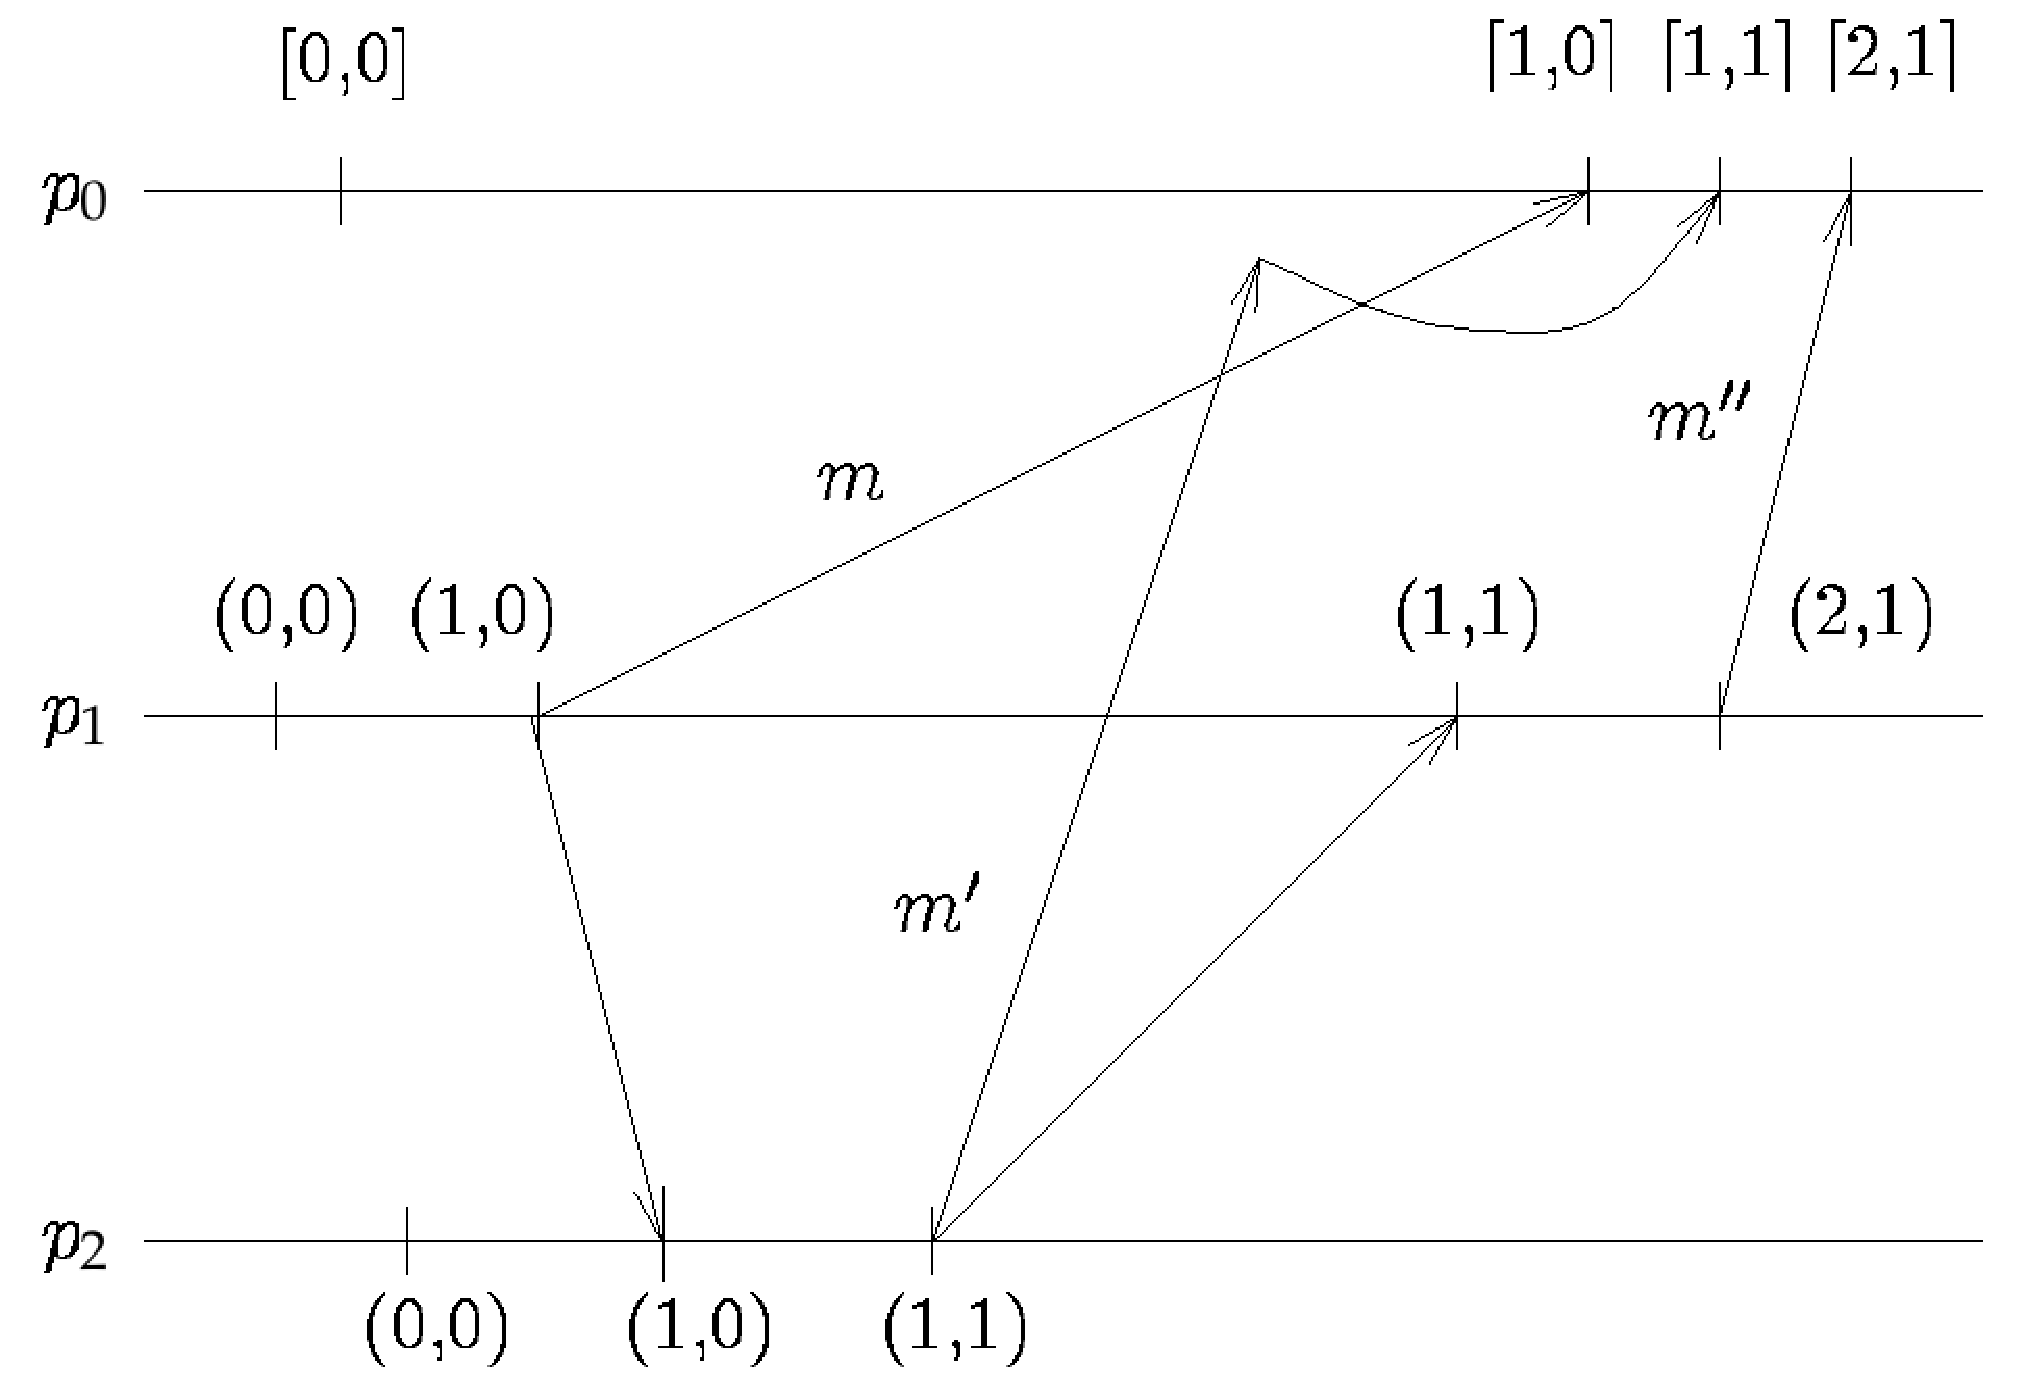
\includegraphics[width=9cm]{figs/03/figure-8}
\end{figure}
\end{frame}

\begin{frame}{Final Comments}
\BIL
\item We have seen how to implement Causal Delivery ``many-to-one'' 
\item The same rules apply if we implement a mechanism for 
  implementing ``one-to-many'' (reliable broadcast)
\EIL
\end{frame}

\section{Proactive monitoring}

\begin{frame}{Snapshot Protocol}

\structure{Problem}
\BI
\item \alert{Goal}:
To build the global state “on demand” of the monitor.
\item \alert{How}:
By taking ``pictures'' (snapshots) of the local state when instructed
\item \alert{Challenge}:
To build a consistent global state.
\EI

\structure{Applications}
\BI
\item Failure recovery: a global state (\alert{checkpoint}) is periodically saved; 
  to recover from a failure, the system is restored to the last saved
  checkpoint.
\item Distributed garbage collection
\item Monitoring distributed events (e.g., industrial process control)
\EI
\end{frame}

\begin{frame}{Chandy and Lamport Snapshot Algorithm}

\BI
\item This particular protocol enables to reason about ``channel states''
\item GPE can be delayed with respect to passive monitoring
\item Assumption: processes communicate through FIFO channels
\EI

\end{frame}

\begin{frame}{Snapshot Protocol}

\begin{block}{Channel State}
\BIL
\item For each channel between $p_i$ and $p_j$
  \BI
    \item $x_{i,j}$ contains the messages sent by $p_i$ but not received yet by $p_j$ 
    \item $x_{j,i}$ contains the messages sent by $p_j$ but not received yet by $p_i$ 
  \EI
\item Note: channel state can be obtained by storing appropriate information
  in the local state, but it is complicated.
\EIL
\end{block}

\bigskip
\begin{block}{Recorded information}
Each process will record its local state $\sigma_i$ and the content of its
\alert{incoming} channels $x_{j,i}$.
\end{block}

\end{frame}

\begin{frame}{Snapshot Protocol}

\structure{Assumptions}:
\BIL
\item Communication channels satisfy FIFO order
\EIL

\bigskip
\structure{Assumptions to be relaxed later}:
\BIL
\item Access to a real time clock $\RC$;
\item Message delays are bounded by some known value $\delta$;
\item Relative process speeds are bounded;
\item Message $m$ is tagged with a timestamp $\TS(m) = \RC(e)$, where $e = \send(m)$.
\EIL
\end{frame}

\subsection{Snapshot protocol, v.1}

\begin{frame}{Snapshot Protocol, v.1}

\BEL
\item $p_0$ chooses a time $t_s$ far enough in the future that a message containing $t_s$
  sent by $p_0$ will be received by all processes by $t_s$:
  \[
     t_s = now() + \delta
  \]
\item $p_0$ sends a message \emph{``take a snapshot at $t_s$''} to all processes in $\Pi$
\item When $\RC_i=t_s$ do:
  \BE
  \item $p_i$ records its local state
  \item $p_i$ sends an empty message to all processes in $\Pi$
  \item $p_i$ starts to record all messages received over each incoming channel
  \EE
\item When $p_i$ receives a message $m$ from $j$ such that $\TS(m) \geq t_s$, it stops recording
  messages for incoming channel $j$
\item Each $p_i$ sends its recorded local state and channel states to $p_0$
\EEL

\end{frame}

\begin{frame}{Snapshot Protocol, v.1}
	
\structure{Liveness} The empty messages at 3.3 guarantee liveness.

\structure{Safety} This protocol constructs a consistent global state;
  actually, this global state did in fact occur. Formally:

Let $C_s$ be the cut associated to the constructed global state;
\begin{eqnarray*}
(e \in C_s) \wedge (e' \rightarrow e) &\Rightarrow& \\
(e \in C_s) \wedge (\RC(e') < \RC(e)) &\Rightarrow& \quad \mbox{C.C.}:  e' \rightarrow e  \Rightarrow \RC(e') < \RC(e) \\
(e' \in C_s) && \quad C_s\ \mbox{Def.}: e \in C_s \Leftrightarrow \RC(e) < t_s 
% e \in C_s \Leftrightarrow \RC(e) < t_s &\quad& \Rightarrow \\
% (e \in C_s) \wedge (\RC(e') < \RC(e)) \Rightarrow (e' \in C_s) &\quad& \\
% e \rightarrow e' \Rightarrow \RC(e') < \RC(e) &\quad& \Rightarrow\\
% (e \in C_s) \wedge (e \rightarrow e') \Rightarrow (e' \in C_s)
\end{eqnarray*}

\structure{Can we use logical clocks instead of a real time clock?}~

\end{frame}

\subsection{Snapshot protocol, v.2}


\begin{frame}{Snapshot Protocol, v.2}

\structure{From real time clocks to logical clocks}:

\BIL
\item The construct ``~{\bf when} $\LC=t_s$ {\bf do} $\mathit{statement}$'' makes no sense
  \BI
  \item $\LC$s are not continuous (e.g., they can jump from $t_s-1$ to $t_s+1$)
  \item When $LC=t_s$, the event that caused the clock update is already done.
  \EI
\item  Solution: before $p_i$ executes an event $e$:
  \BI
  \item If $e$ is an internal or send event, and $\LC = t_s-2$:
    \BI
      \item $p_i$ executes $e$
      \item $p_i$ executes $\mathit{statement}$
    \EI
  \item If $e=\receive(m) \wedge \TS(m) \geq t_s$ and $\LC < t_s-1$:
	\BI
	\item $p_i$ puts $\LC=t_s-1$
	\item $p_i$ executes $\mathit{statement}$
	\item $p_i$ executes $e$
	\EI
  \EI
\EIL

\end{frame}



\begin{frame}{Snapshot Protocol, v.2}

\structure{From real time clocks to logical clocks}:

\BI
\item We assume that we can found a logical time $t_s$ large
  enough that a message containing it sent by $p_0$ will be 
  received by all other processes before $t_s$
\item Impossible in an asynchronous distributed systems
\item We will relax this assumption later
\EI
\end{frame}

\begin{frame}{Snapshot Protocol, v.2}
\BEL
\item $p_0$ chooses a logical time $t_s$ large enough
\item $p_0$ sends a message \emph{``take a snapshot at $t_s$''} to all processes in $\Pi$
\item $p_0$ sets its logical clock to $t_s$;
\item When $\LC_i=t_s$ do:
  \BE
  \item $p_i$ records its local state;
  \item $p_i$ sends an empty message to all processes in $\Pi$;
  \item $p_i$ starts to record all messages received over each incoming channel.
  \EE
\item When $p_i$ receives a message $m$ from $j$ such that $\TS(m) \geq t_s$, it stops recording
  messages for incoming channel $j$
\item Each $p_i$ sends its recorded local state and channel states to $p_0$.
\EEL
\end{frame}

\subsection{Snapshot protocol, v.3}

\begin{frame}{Snapshot Protocol, v.3}

We now remove the need for $t_s$:

\BIL
\item A process may receive an "empty message" from a node before the ``take
snapshot at $t_s$'' is actually received
\item In other words, it may be already aware of the snapshot protocol
\item We remove the ``at $t_s$'' and we use \SNAPSHOT messages instead of
empty ones
\item We can now remove logical clocks completely, as messages are not
timestamped any more
\EIL

\end{frame}

\begin{frame}{Snapshot Protocol, v.3}
	
\BEL
\item $p_0$ sends a message \SNAPSHOT to itself ;
\item when $p_i$ receives \SNAPSHOT for the \alert{first time}:
  \BI 
  \item let $p_j$ be the sender of this message
  \item $p_i$ records its local state $\sigma_i$;
  \item sends \SNAPSHOT to all processes in $\Pi$;
  \item $x_{k,i} \gets \emptyset \qquad \forall k \neq i$;
  \EI
\item when $p_i$ receives message $m \neq$ \SNAPSHOT from $p_k, k \neq j$
  \BI
  \item $x_{k,i} \gets x_{k,i} \cup \{ m \}$
  \EI
\item when $p_i$ receives a \SNAPSHOT from
  $p_k, k \neq j$ beyond the \alert{first time}:
  \BI
  \item $p_i$ stops recording messages in $x_{k,i}$;
  \EI
\item when $p_i$ has received a \SNAPSHOT
  from all processes
  \BI
  \item $p_i$ then sends its recorded local state and the channel states to $p_0$.
  \EI
\EEL

\end{frame}

\begin{frame}{Example}
\begin{figure} 
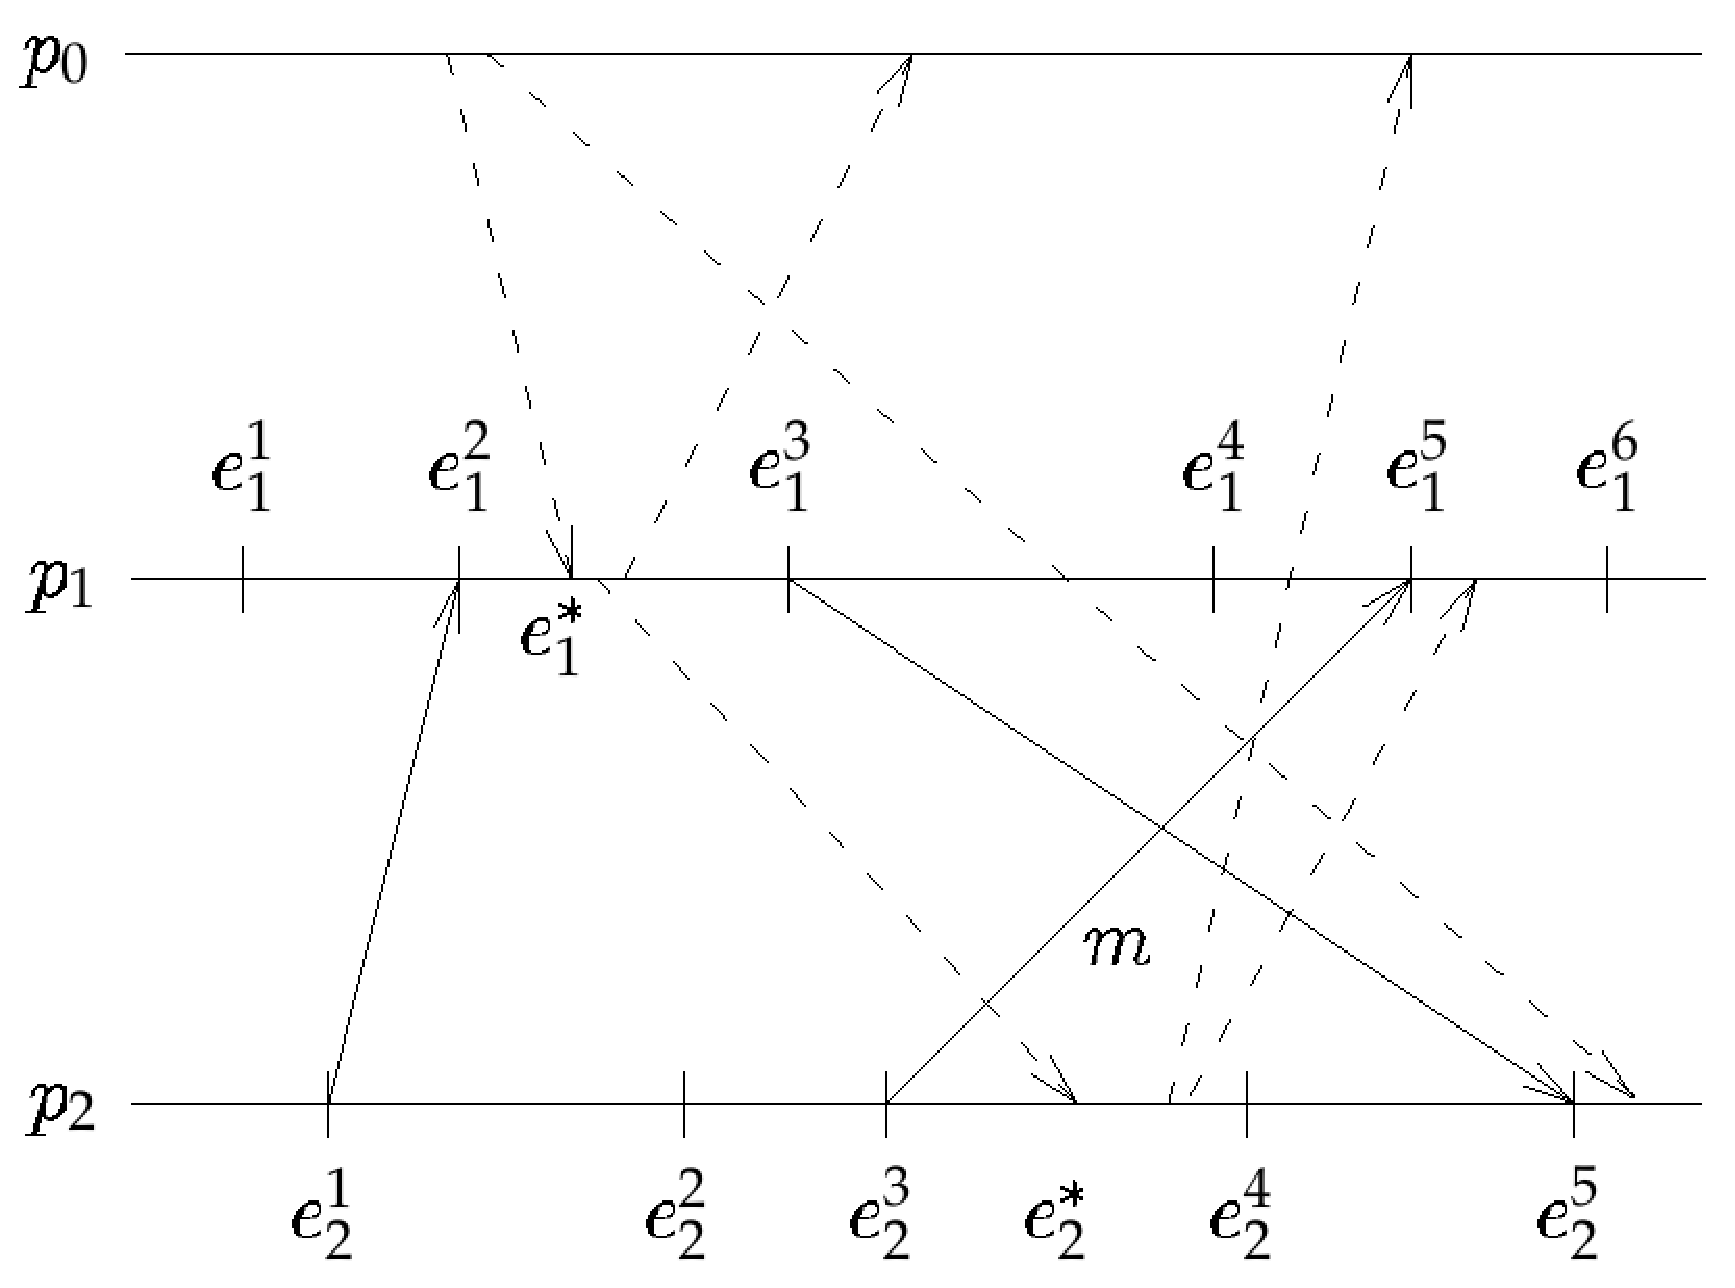
\includegraphics[width=9cm]{figs/03/figure-10}
\end{figure}
\end{frame}

\begin{frame}{Proof of correctness}
	
\begin{theorem}
A global state built using the Chandy-Lamport snapshot algorithm is consistent.
\end{theorem}
\end{frame}


\note{

In order for the global state to be inconsistent, there should be a 
receive event included in the global state for which the corresponding
send event is not included. Let $e_i = \receive_i(m)$ and let $e_j = \send_j(m)$.

In order for $e_j$ to not belong to the global state, process $p_j$ must 
have received the first \SNAPSHOT message before $e_j$. Thus, it has sent a message to 
$p_i$ containing a $\SNAPSHOT$ message to $p_i$ before sending $m$. For the
FIFO property of the channel, $p_i$ must have received the $\SNAPSHOT$ message
before $e_i$. So, it must have stored the local state before receiving $m$,
a contradiction.

}


\section{Stable predicates}


\begin{frame}{Stable Predicates}

\begin{block}{Problem}
\BI
\item Let $\Sigma$ be a global state built by one of the methods presented
\item It represents a state of the past, potentially with no bearing to the present
\item Does it make sense to evaluate predicate $\Phi$ on it?
\EI
\end{block}

\begin{block}{A special case: stable predicates}

Many systems properties have the characteristic that once they become true, they remain true.
\BI
\item Deadlock
\item Garbage collection
\item Termination
\EI
\end{block}

\end{frame}

\begin{frame}{A distributed computation may have many runs}

\begin{definition}[Leads-to relation]
\BIL
\item A consistent run $R=e^1 e^2 \ldots$ results in a sequence of consistent global states
$\Sigma^0 \Sigma^1 \Sigma^2 \ldots$, where $\Sigma^0$ denotes the initial global state.
\item We say that a global state $\Sigma$ \alert{leads to} to a global state $\Sigma'$, denoted
  $\Sigma \leadsto_R \Sigma'$ in a consistent run $R$ if:
  \BI 
  \item $R$ results in a sequence of global states $\Sigma^0 \Sigma^1 \Sigma^2 \ldots$;
  \item $\Sigma = \Sigma^i, \Sigma' = \Sigma^j, i < j$.
  \EI
\item We write $\Sigma \leadsto \Sigma'$ if there is a run $R$ such that $\Sigma \leadsto_R \Sigma'$.
\EIL
\end{definition}

\end{frame}

\begin{frame}{A distributed computation may have many runs}
	
\begin{definition}[Lattice]
\BIL
\item The set of all consistent global states of a computation along with the leads-to relation
defines a \alert{lattice};
\item $n$ orthogonal axis, one per process;
\item $\Sigma^{k_1 \ldots k_n}$ shorthand for the global state $(\sigma_1^{k_1}, \ldots, \sigma_n^{k_n})$;
\item The \alert{level} of $\Sigma^{k_1 \ldots k_n}$ is equal to $k_1+ \cdots + k_n$.
\item A path in the lattice is a sequence of global states of increasing levels that corresponds
  to a consistent run.
\EIL
\end{definition}

\end{frame}

\begin{frame}
\begin{figure} 
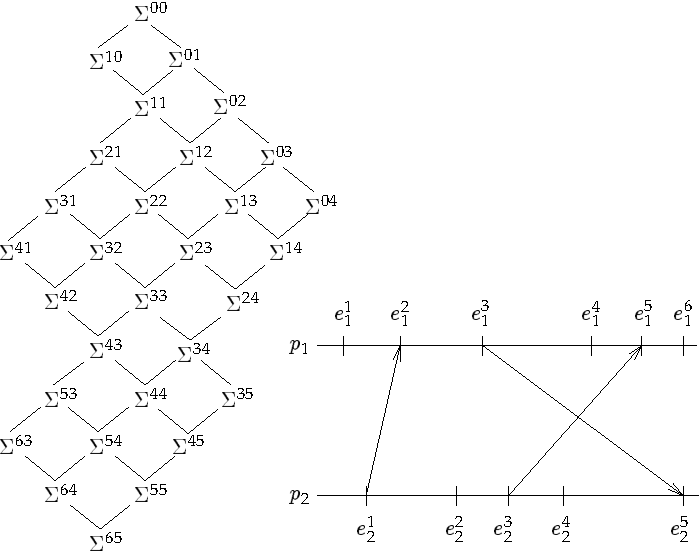
\includegraphics[width=9.5cm]{figs/03/figure-3}
\end{figure}
\end{frame}


\begin{frame}{Stable Predicates}

Consider a global state construction protocol:
\BI
\item Let $\Sigma^a$ be the global state in which the protocol is initiated;
\item Let $\Sigma^f$ be the global state in which the protocol terminates;
\item Let $\Sigma^s$ be the global state constructed by the protocol
\EI
Since $\Sigma^a \leadsto \Sigma^s \leadsto \Sigma^f$, if $\Phi$ is stable, then:
\begin{eqnarray*}
\Phi(\Sigma^s) = \mathbf{true} &\Rightarrow& \Phi(\Sigma^f) = \mathbf{true} \\
\Phi(\Sigma^s) = \mathbf{false} &\Rightarrow& \Phi(\Sigma^a) = \mathbf{false}
\end{eqnarray*}

\end{frame}

\subsection{Deadlock detection}

\begin{frame}{Deadlock Detection}

\structure{Code}
\BI 
\item Server code
\item Server code, modified for snapshot protocol
\item Monitor code for snapshot protocol
\item Server code, modified for passive protocol
\item Monitor code for passive protocol
\EI

\structure{Notes}
\BI
\item No need to store channel state in this case
\EI

\end{frame}


\begin{frame}[shrink]{Server code}

\begin{Procedure}
\caption{Process\ $p_i$}
  $\Queue\ \Pending \gets \NEW\ \Queue()$\;
  $\BOOLEAN\ \Working \gets \FALSE$\;
  \While{\TRUE}{
	\While{$\Working$ \OR $\Pending.\Size() = 0$}{
	  \RECEIVE $\langle m, p_j \rangle$\;
	  \uIf{$m.\Type = \REQUEST$}{
	    $\Pending.\Enqueue(\langle m, p_j \rangle)$\;
	  }\ElseIf{$m.\Type = \RESPONSE$}{
	    $\langle m', p_k \rangle \gets \NextState(m,p_j)$\;
	    $\Working \gets (m'.\Type = \REQUEST)$\;
	    \SEND $m'$ \TO\ $p_k$\;
	  } 
	}
	\While{\NOT $\Working$ \AND $\Pending.\Size() > 0$}{
	  $\langle m, p_j \rangle \gets \Pending.\Dequeue()$\;
	  $\langle m', p_k \rangle \gets \NextState(m,p_j)$\;
	  $\Working \gets (m'.\Type = \REQUEST)$\;
	  \SEND $m'$ \TO\ $p_k$\;
	}
  }
\end{Procedure}

\end{frame}

\subsection{Deadlock detection through active monitoring}

\begin{frame}{Deadlock Detection through Snapshot}

\structure{Approach}
\BI
\item All channels are based on FIFO delivery
\item Add code to deal with Snapshot messages
\EI

\bigskip
\structure{Pros and Cons}
\BI
\item Generates overhead only when deadlock is suspected
\item Introduces a delay between deadlock and detection
\EI


\end{frame}

\begin{frame}[shrink]{Server code, modified for active monitoring (1)}

%% TODO: Sistemare l'uwhile (ma perchè non esiste?)

\begin{Procedure}
\caption{Process\ $p_i$}
  $\Queue\ \Pending \gets \NEW\ \Queue()$\;
  $\BOOLEAN\ \Working \gets \FALSE$\;
  $\color{red} \BOOLEAN[]\ \Blocking \gets \{ \FALSE, ..., \FALSE \}$\;
  \uWHILE{\TRUE}{
    \uWHILE{$\Working$ \OR $\Pending.\Size() = 0$}{
      \RECEIVE $\langle m, p_j \rangle$\;
      \uIf{$m.\Type = \REQUEST$}{
        $\color{red}\Blocking[j] \gets \TRUE$\;
        $\Pending.\Enqueue(\langle m, p_j \rangle)$\;
      }
      \ElseIf{$m.\Type = \RESPONSE$}{
        $\langle m', p_k \rangle \gets \NextState(m,p_j)$\;
        $\Working \gets (m'.\Type = \REQUEST)$\;
        \SEND $m'$ \TO\ $p_k$\;
        {\color{red}
          \If{$m'.\Type = \RESPONSE$}{
             $\Blocking[k] \gets \FALSE$\;
          }
        }
      } 
    }
  }
\end{Procedure}

\end{frame}

\begin{frame}[shrink]{Server code, modified for active monitoring (2)}

\begin{Procedure}
\caption{Process\ $p_i$}
\UNVISIBLE{}{
{\color{red}
\UNVISIBLE{}{
\ElseIf{$m.\Type = \SNAPSHOT$}{
  \If{$s=0$}{
    \SEND $\langle \SNAPSHOT, \Blocking \rangle$ \TO $p_0$\;
    \SEND $\langle \SNAPSHOT \rangle$ \TO $\Pi - \{ p_i \}$\;
  }
  $s \gets (s+1) \bmod n$\;
}
}
}
\While{\NOT $\Working$ \AND $\Pending.\Size() > 0$}{
  $\langle m, p_j \rangle \gets \Pending.\Dequeue()$\;
  $\langle m', p_k \rangle \gets \NextState(m,p_j)$\;
  $\Working \gets (m'.\Type = \REQUEST)$\;
  \SEND $m'$ \TO $p_k$\;
  {\color{red}
    \If{$m'.\Type = \RESPONSE$}{
      $\Blocking[k] \gets \FALSE$\;
    }
  }
}
}
\end{Procedure}

\end{frame}

\begin{frame}{Monitor code, for active monitoring}
	
\begin{Procedure}
\caption{Process\ $p_0$}
  $\BOOLEAN[\,][\,]\ \Wfg \gets \NEW\ \BOOLEAN[1 \ldots n][1 \ldots n]$\;
  \While{\TRUE}{
    \{ Wait until deadlock is suspected \}\;
    \SEND $\langle \SNAPSHOT \rangle$ \TO $\Pi$\;
    \For{$k \gets 1$ \TO $n$}{
       \RECEIVE $\langle m, j \rangle$\;
       $\Wfg[j] \gets m.\Data$\;
    }
    \If{there is a cycle in $\Wfg$}{
      \{ the system is deadlocked \}\;
    }
  }
\end{Procedure}

\end{frame}

\subsection{Deadlock detection through passive monitoring}

\begin{frame}{Deadlock detection through passive monitoring}

\structure{Approach}
\BI
\item Sends a message to $p_0$ for each relevant event
\item Communication with $p_0$ based on causal delivery
\EI

\bigskip
\structure{Pros and Cons}
\BI
\item Simpler approach, but complexity is hidden by the
  causal delivery mechanism
\item Latency limited to message delays
\item Higher overhead
\EI


\end{frame}


\begin{frame}[shrink]{Server code, modified for passive monitoring}

\begin{Procedure}
\caption{Process\ $p_i$}
  $\Queue\ \Pending \gets \NEW\ \Queue()$\;
  $\BOOLEAN\ \Working \gets \FALSE$\;
  \While{\TRUE}{
    \While{$\Working$ \OR $\Pending.\Size() = 0$}{
      \RECEIVE $\langle m, p_j \rangle$\;
      \uIf{$m.\Type = \REQUEST$}{
        {\color{red} \SEND $\langle \REQUESTED, j, i \rangle$ \TO $p_0$}\;
        $\Pending.\Enqueue(\langle m, p_j \rangle)$\;
      }
      \ElseIf{$m.\Type = \RESPONSE$}{
        $\langle m', p_k \rangle \gets \NextState(m,p_j)$\;
        $\Working \gets (m'.\Type = \REQUEST)$\;
        \SEND $m'$ \TO\ $p_k$\;
        {\color{red}
          \If{$m'.\Type = \RESPONSE$}{
             {\color{red} \SEND $\langle \RESPONDED, i, k \rangle$ \TO $p_0$}\;
          }
        }
      } 
      \While{\NOT $\Working$ \AND $\Pending.\Size() > 0$}{
        $\langle m, p_j \rangle \gets \Pending.\Dequeue()$\;
        $\langle m', p_k \rangle \gets \NextState(m,p_j)$\;
        $\Working \gets (m'.\Type = \REQUEST)$\;
        \SEND $m'$ \TO $p_k$\;
		{\color{red}
        \If{$m'.\Type = \RESPONSE$}{
            \SEND $\langle \RESPONDED, i, k \rangle$ \TO $p_0$\;}
        }
     }
    }
  }
\end{Procedure}

\end{frame}

\begin{frame}[shrink]{Monitor code, for passive monitoring}

\begin{Procedure}
\caption{Process\ $p_0$}
  $\BOOLEAN[\,][\,]\ \Wfg \gets \NEW\ \BOOLEAN[1 \ldots n][1 \ldots n]$\;
  \While{\TRUE}{
    \RECEIVE $\langle m,p_j \rangle$\;
    \eIf{$m.\Type = \RESPONDED$}{
      $\Wfg[m.\From, m.\To] \gets \FALSE$\;
    }{
      $\Wfg[m.\From, m.\To] \gets \TRUE$\;
    }
    \If{there is a cycle in $\Wfg$}{
      \{ the system is deadlocked \}\;
    }
  }
\end{Procedure}
\end{frame}

\section{Non-stable predicates}

\begin{frame}{Non-stable predicates}
	
\structure{Problems of non-stable predicates}

\BI
\item The condition encoded by the predicate may not persist long enough for it to 
  be true when the predicate is evaluated
\item If a predicate $\Phi$ is found to be true by the monitor, we do not know whether 
  $\Phi$ \emph{ever} held during the \emph{actual} run.
\EI

\bigskip
\structure{Conclusions}

\BI
\item Evaluating a non-stable predicate over a single computation makes no sense
\item The evaluation must be extended to the entire lattice of the computation
\EI

\end{frame}

\begin{frame}{Predicates over entire computations}
	
It is possible to evaluate a predicate over an entire computation using
an observation obtained by a passive monitor.

\BI
\item \alert{{\bf Possibly}($\Phi$)}: There exists a consistent observation $O$ 
  of the computation such that $\Phi$ holds in a global state of $O$.
\item \alert{{\bf Definitely}($\Phi$)}: For every consistent observation $O$ of
  the computation, there exists a global state of $O$ in which $\Phi$ holds.
\EI

\begin{example}[Debugging]
If {\bf Possibly}($\Phi$) is true, and $\Phi$ identifies some erroneous state of the
computation, than there is a bug, even if it is not observed during an actual run.
\end{example}

\end{frame}


\begin{frame}

\structure{Example}: {\bf Possibly}($(y-x)=2$), {\bf Definitely}($x=y$)
\begin{figure} 
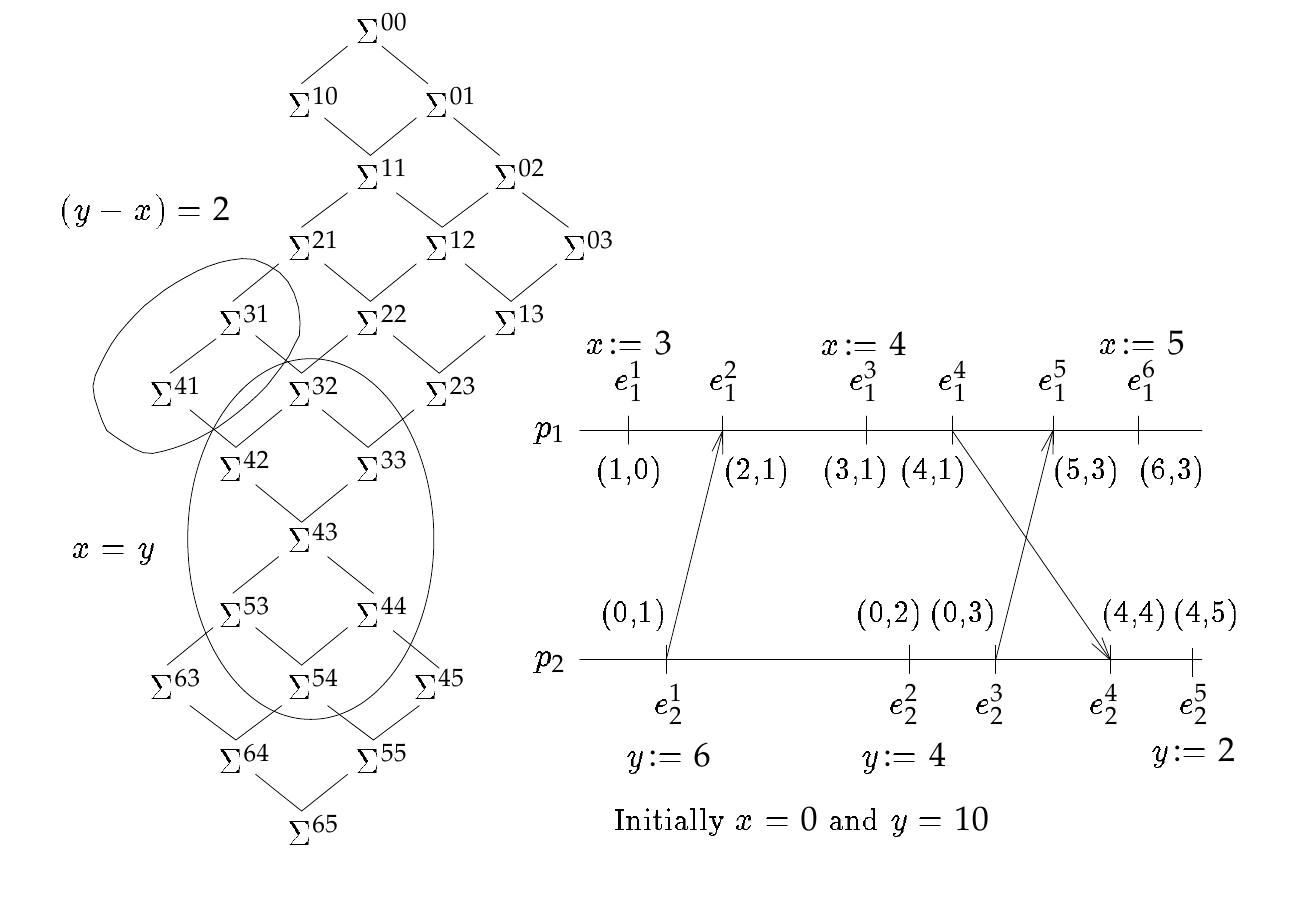
\includegraphics[width=10cm]{figs/03/figure-16.png}
\end{figure}
\end{frame}

\begin{frame}{Predicates over entire computations}

\begin{theorem}
{\bf Possibly} and {\bf Definitely} are not duals:
\begin{eqnarray*}
\neg \mathbf{Possibly}(\Phi) &\not\Leftrightarrow& \mathbf{Definitely}(\neg \Phi) \\
\neg \mathbf{Definitely}(\Phi) &\not\Leftrightarrow& \mathbf{Possibly}(\neg \Phi)
\end{eqnarray*}
\end{theorem}

\bigskip
\begin{example}
{\bf Possibly}($x \neq y$), {\bf Definitely}($x=y$)
\end{example}

\end{frame}

\begin{frame}{Algorithms for detecting {\bf Possibly} and {\bf Definitely}}

\BI
\item We use the passive approach in which processes send notifications of events 
  relevant to $\Phi$ to the monitor $p_0$;
\item Events are tagged with vector clocks; 
\item The monitor collects all the events and builds the lattice of global
  states.\\
  {\bf How?}
\item To detect {\bf Possibly}($\Phi$): if there exists one 
  global state in which $\Phi$ is true, then return {\bf true}, otherwise
  {\bf false}.
\item To detect {\bf Definitely}($\Phi$): mark nodes where $\Phi$ is true
  with a value $1$, the other nodes with value $0$. If the cost of the 
  shortest path between the initial state and the final state is larger
  than $0$, return {\bf true}, otherwise
  {\bf false}.
\EI

\end{frame}

\begin{frame}{Algorithms for detecting {\bf Possibly} and {\bf Definitely}}

\structure{Problems}
\BIL
\item The number of states grows exponentially with the number of total
  events. 
\item Techniques can be used to reduce the number of events
\BI
\item Only those relevant to $\Phi$
\item Forcing periodic synchronization
\item Reducing the complexity of predicates (conjunction of local predicates)
\EI
\EIL

\end{frame}

\nocite{ozalp93consistent}

\begin{frame}{Reading material}

{\footnotesize
\bibliographystyle{abbrv}
\bibliography{../references}  
}

\end{frame}


\end{document}

